\begin{SingleSpace}
\chapter{Wave-Mean Flow Interactions in a Linear Theory of Tidally Locked Atmospheres}\label{ch:wave-mean-flow}
\vspace{0.5cm}
\chapterprecishere{``One might as well approximate the derivatives well instead of badly''\par\raggedleft--- \textup{John P. Boyd}, Chebyshev and Fourier Spectral Methods}
\end{SingleSpace}
\vspace{0.5cm}

%0 -- LEAD-IN PARAGRAPHS

%START ELEMENT
Tidally locked planetary atmospheres have such a different spatial energy input to planets like the Earth that it is not obvious that conventional Earth-like atmospheric dynamics should be able to describe them. However, the planetary-scale day-night forcing difference makes the global circulation highly susceptible to a simple shallow-water model, compared to the higher order effects controlling the Earth's atmosphere.

%FRAMING TEXT
This chapter discusses my work using a single-layer linear shallow-water model to investigate the global circulation of tidally locked planets. It follows directly from the work of XX and XX. As introduced in Chapter \ref{ch:lava-planets}, the atmospheres of tidally locked planets are understood to generally have a strong eastward equatorial jet, a hot-spot shifted eastward of their substellar point, and a pair of cold low-pressure lobes on their night-side. Figure \ref{fig:example-gcm-results} shows a GCM simulation of a tidally locked planet with Earth-like size and instellation, showing these features.

In this chapter, I will show that the interaction of this mean zonal flow and the standing waves produced by the stationary day-night forcing is crucial to the global circulation of tidally locked planets. \citet{showman2011superrotation} used a shallow-water model to model the standing waves on tidally locked planets, and to explain the equatorial superrotation. However, the equilibrium state of their shallow-water model only matched the form of their GCM simulations over the first few days after spin-up from rest. \citet{tsai2014three} suggested that this was because the zonal flow shifted the standing wave response eastwards, and used a uniform flow (with no height perturbation) in a shallow-water model to show this. In this chapter, I follow both of these studies and linearise the shallow-water equations around a meridionally sheared zonal flow $\bar{U}(y)$ with an associated height perturbation $\bar{H}(y)$. I show that the response to day-night forcing in this system matches GCM simulations of tidally locked planets, particularly the form of the hot-spot shift and the cold lobes on the night-side.

\begin{figure}
  \centering
  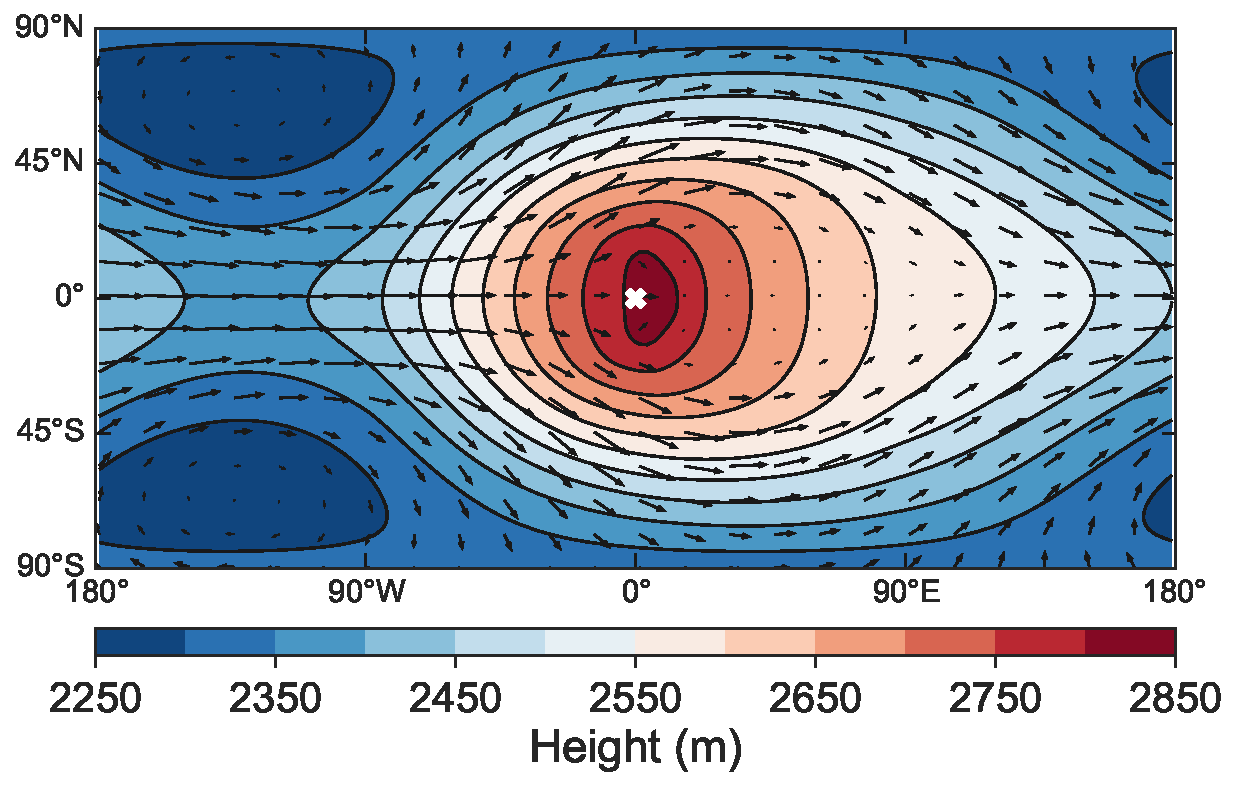
\includegraphics[width=0.6\textwidth]{figures/wave-mean-flow/example-gcm-results.pdf}
  \caption{Example GCM results.}
  \label{fig:example-gcm-results}
\end{figure}

%SIGNPOSTS
After introducing the linear shallow-water model and the work of Matsuno, Gill, Showman, and Tsai, I will show how I linearised the model about a zonally uniform jet $\bar{U}(y)$ with latitudinal shear, as well as its associated geostrophic height perturbation $\bar{H}(y)$.

In Section 1, I will introduce the system of shallow-water equations on a rotating beta-plane, and discuss the response to a day-night forcing, in zero background flow and in uniform background flow (an approximation to the later shear flow and height perturbation).

In Section 2, I will show the zonal acceleration produced by this forced response, discussing how \citet{showman2010superrotation} showed that a correction to the classical model of \citet{matsuno1966quasi} is required to produce equatorial superrotation.

In Section 3, I will linearise the beta-plane shallow-water equations about a background flow $\bar{U}(y)$ and associated height perturbation $\bar{H}(y)$, representing the flow produced by this acceleration. I will find the free modes of this system and the response to the same day-night forcing as before. This will show that the forced response is shifted eastwards, combining with the zonally uniform jet perturbation to produce the global circulation pattern seen in GCM simulation and hinted at by observations.

In Section 4, I will show the same calculation for the shallow-water equations on a sphere, which have less intuitive solutions but are more directly comparable to real planets and GCM simulations.

In Section 5, I will use the shallow-water equations to produce simple one-dimensional scaling relations for the height field along the equator, and compare them to the two-dimensional scaling relations predicted by the solutions in the previous sections.

In the next chapters, I will return to these stationary solutions and scaling relations  to compare them to GCM simulations.

%%%%%


%SUMMARISE CONCLUSIONS
I will show that linearising the jet about the shear flow and its height perturbation makes the forced linear response match nonlinear GCM simulations much more closely. The new model reveals scaling relations between the planetary parameters such as forcing strength, and the observable quantities such as the eastward hot-spot shift.

This chapter is based on work produced for \citet{hammond2018wavemean}. Some of the figures, which I generated, have been taken directly from this paper. None of the text has been reused, and the structure is significantly different.

%%%%%%%%%%%%%%%%%%%%%%%%%%%%%%%%%%%%


%SECTION 1 -- LINEAR SHALLOW-WATER AND UNIFORM FLOW
\section{The Shallow-Water Equations}\label{sec:shallow-water}

We used the linear shallow-water equations on a one-layer equatorial beta-plane to model the atmosphere of a tidally locked planet. These equations describe the motion of a single layer of fluid of constant density where the horizontal scale of its flow is much greater than the depth of the fluid. The linear form of these equations describe small perturbations to this layer \citep{vallis2006book}. We model the atmosphere of a tidally locked planet with a similar shallow-water model to \citet{showman2011superrotation}. The model corresponds to an active upper layer following the single-layer shallow water equations, above a quiescent layer which can transport mass and momentum to and from the upper layer. The forcing due to stellar heating is represented by $Q$, a relaxation to the radiative equilibrium height field.

%SUBSECTION -- LINEAR SHALLOW-WATER
\subsection{Free Solutions}

In this section, we derive the wave response to stationary forcing on the beta-plane \citep{matsuno1966quasi}. The beta-plane system approximates the Coriolis parameter as linear, which is only accurate at low latitudes but leads to more intuitive and useful solutions than the full spherical geometry. We solve the equations in a spherical geometry in Section \ref{sec:sphere-solutions}, and show that the beta-plane approximation leads to very similar solutions, as in other studies of the atmospheres of tidally locked planets \citep{showman2011superrotation} \citep{heng2014analytical}.

All the quantities are linearized as the sum of a zonally mean background value $F(y)$  and a perturbation with the form  $f(y) e^{i( k_{x} x-\omega t)}$ (unlike \citet{matsuno1966quasi}, who uses the less conventional form  $f(y) e^{i( k_{x} x+\omega t)}$). Throughout this paper, we will use capital letters for mean zonal quantities such as $\bar{U}$ and $\bar{H}$, and lower-case letters for perturbations to this background, such as $u$ and $h$ (unless otherwise specified, such as the forcing $Q$). The shallow-water equations for these perturbations with zero background flow are:

\begin{equation}\label{eqn:sw-eqns-1}
  \begin{gathered}
     \frac{\partial u}{\partial t} - \beta y v +\frac{\partial h}{\partial x} = 0 \\
      \frac{\partial v}{\partial t} + \beta y u + \frac{\partial h}{\partial y} = 0 \\
    \frac{\partial h}{\partial t} +c^{2}(\frac{\partial u}{\partial x} + \frac{\partial v}{\partial y}) = Q(x,y) \\
  \end{gathered}
\end{equation}

where $h$ is the height, $c = \sqrt{gH}$ is the gravity wave speed \citep{matsuno1966quasi}, and there is no friction or damping. Non-dimensionalizing with time scale $\sqrt{1/c \beta}$ and length scale $\sqrt{c/\beta}$ (the equatorial Rossby radius of deformation $L_{R}$), and assuming all quantities have the form $f(y) e^{i( k x-\omega t)}$, the free equations with zero forcing are:

\begin{equation}\label{eqn:sw-eqns-2}
  \begin{gathered}
      - i \omega u - y v + i k_{x} h = 0 \\
      - i \omega v + y u + \frac{\partial h}{\partial y} = 0 \\
      - i \omega h + i k u + \frac{\partial v}{\partial y} = 0 \\
  \end{gathered}
\end{equation}

\citet{matsuno1966quasi} gives the free modes of this system as XX. Figure \ref{fig:free-kelvin-mode} shows the free Kelvin mode with wavenumber 1 and Figure \ref{fig:free-rossby-mode} shows the free Rossby mode with wavenumber 1.

EIGENVALUES GIVE POSITION IN FORCED RESPONSE.

\begin{figure}
  \centering
  \begin{subfigure}[b]{0.49\textwidth}
    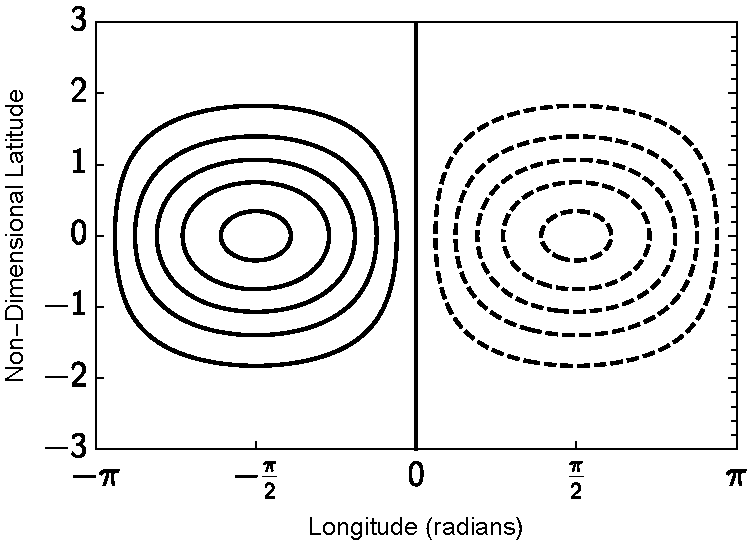
\includegraphics[width=1.0\textwidth]{figures/wave-mean-flow/free-kelvin-mode.pdf}
    \caption{Free Kelvin Mode.}
    \label{fig:free-kelvin-mode}
  \end{subfigure}
  %
  \begin{subfigure}[b]{0.49\textwidth}
    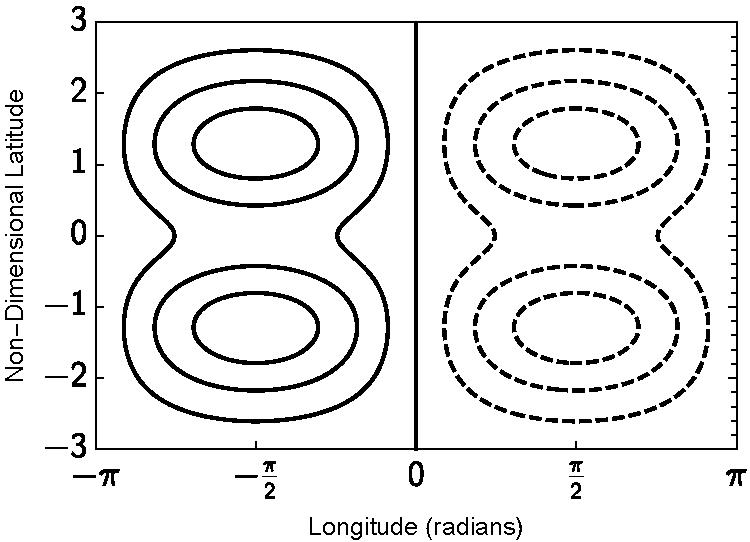
\includegraphics[width=1.0\textwidth]{figures/wave-mean-flow/free-rossby-mode.pdf}
    \caption{Free Rossby Mode.}
    \label{fig:free-rossby-mode}
  \end{subfigure}
  \caption{Free Modes.}
  \label{fig:free-kelvin-rossby-mode}
\end{figure}

%SUBSECTION --
\subsection{Forced Solutions}

In this chapter, I will focus on the response of the shallow-water equations to a forcing $Q(x,y)$ on the height field $h$, representing the stellar forcing on a tidally locked planet. The forced solution can be considered to be a sum of the free modes discussed in the previous section, at different locations and with different strengths.

The forced equations are:

\begin{equation}\label{eqn:sw-eqns-forced}
  \begin{gathered}
    \alpha_{rad} u - \beta y v +\frac{\partial h}{\partial x} = 0 \\
    \alpha_{rad} u + \beta y u + \frac{\partial h}{\partial y} = 0 \\
    \alpha_{dyn} h + c^{2}(\frac{\partial u}{\partial x} + \frac{\partial v}{\partial y}) = Q(x,y) \\
  \end{gathered}
\end{equation}

with boundary conditions

\begin{equation}
  u , v , h \rightarrow 0 \quad \mathrm{for} \quad y \rightarrow \pm \infty.
\end{equation}

\citet{matsuno1966quasi} shows how the response of Equation \ref{eqn:sw-eqns-forced} to a forcing $Q(x,y) = Q_{0} \sin(x) e^{-y^{2}/2}$ and uniform damping $\alpha_{rad}=\alpha_{dyn}=\alpha$ can be found analytically as a sum of the free modes of the system. The forced response $\chi = (u,v,h)$ is a sum of the free modes $\xi_{m}=(u_{m},v_{m},h_{m})$, weighted by coefficients $a_{m}$

\begin{equation}
  \chi = \sum a _ { m } \xi _ { m },
\end{equation}

where the coefficients are given by

\begin{equation}
  a _ { m } = \frac { 1 } { \alpha - i \omega _ { m } } b _ { m },
\end{equation}

where $\omega_{m}$ is the eigenvalue of the mode $m$, and

\begin{equation}
  b _ { m } = \left[ \int \overline { \xi } _ { m } ( y ) \sigma ( y ) d y \right] / \left[ \int \left| \xi _ { m } ( y ) \right| ^ { 2 } d y \right].
\end{equation}

For the forcing $Q(x,y) = Q_{0} \sin(x) e^{-y^{2}/2}$, all of the coefficients $a_{m}$ are zero, apart from those for the Kelvin wave and the $n=1$ Rossby wave. Figure \ref{fig:motivate-showman} shows this forced response.

DO THIS! The eigenvalues determine the position of each free mode in the forced response.

In the rest of this chapter, I willl instead use the pseudo-spectral method described in Appendix \ref{ap:ps-methods} to find the response to forcing. This method works for any forcing and background flow (unlike the analytic method), and still finds the exact analytic solution for this case with zero background flow. Figure \ref{fig:motivate-showman} was actually calculated using this pseudo-spectral method rather than expanding in terms of the free modes, but the solution is identical (as explained in Appendix \ref{ap:ps-methods}, the basis functions of the pseudo-spectral method can exactly represent the free modes of the shallow-water system).

\begin{figure}
  \centering
  \begin{subfigure}[b]{0.49\textwidth}
    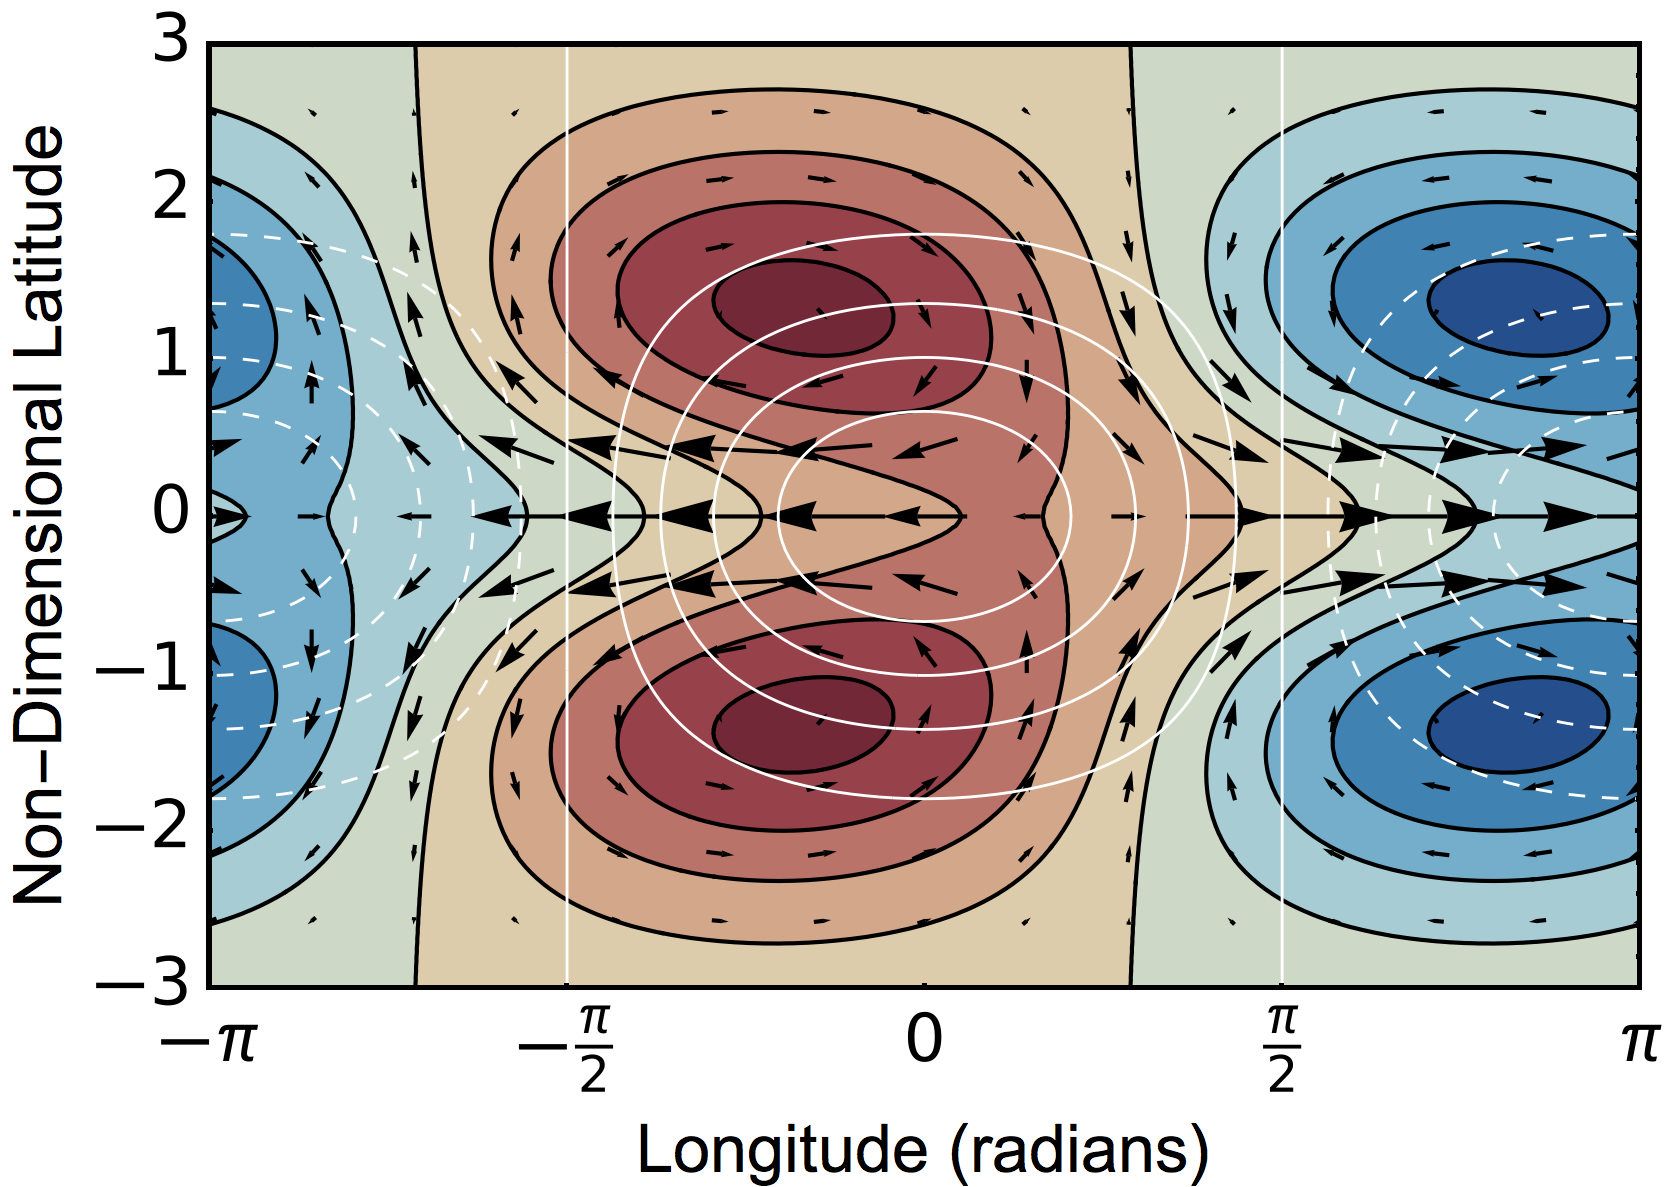
\includegraphics[width=1.0\textwidth]{figures/wave-mean-flow/motivate-showman.png}
    \caption{motivate-showman.}
    \label{fig:motivate-showman}
  \end{subfigure}
  %
  \begin{subfigure}[b]{0.49\textwidth}
    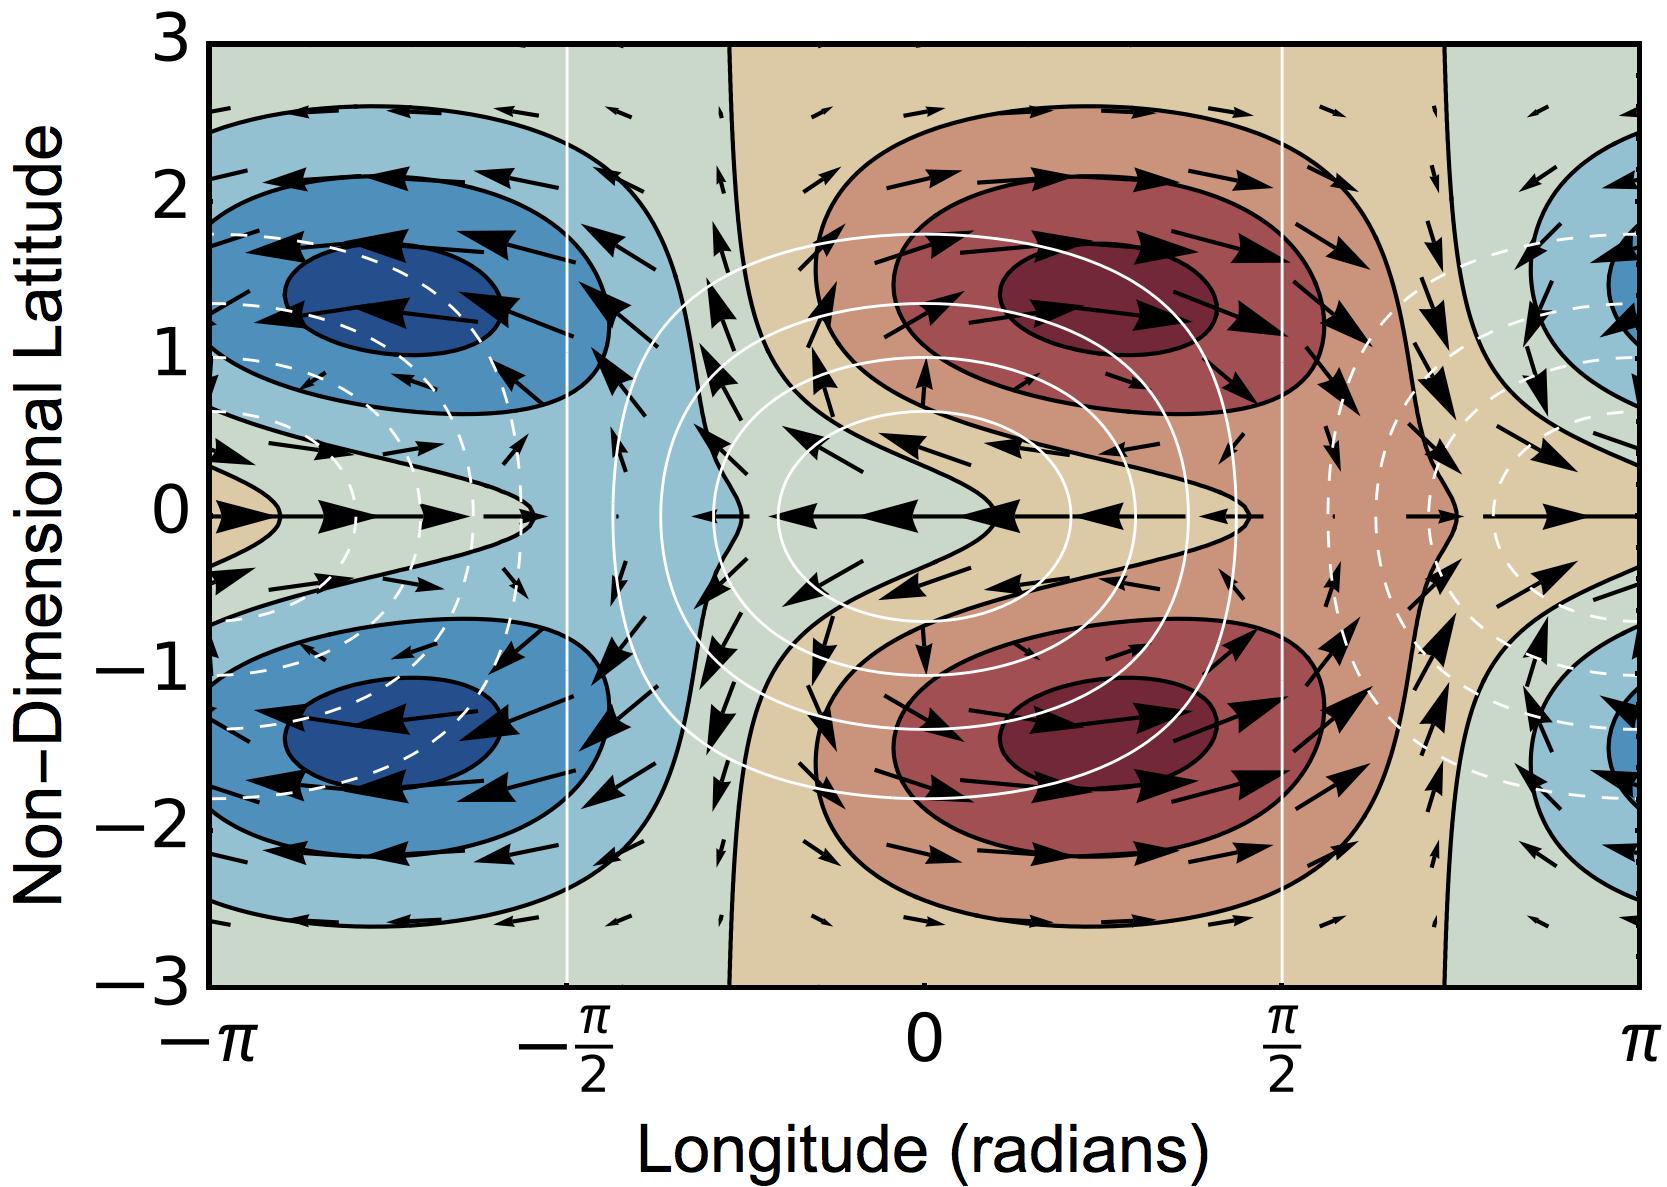
\includegraphics[width=1.0\textwidth]{figures/wave-mean-flow/motivate-tsai.png}
    \caption{motivate-tsai.}
    \label{fig:motivate-tsai}
  \end{subfigure}
  \caption{Forced solutions.}
  \label{fig:motivate-showman-tsai}
\end{figure}


%SUBSECTION -- UNIFORM FLOW
\subsection{Wave Interactions with Flow}

This flow can be approximated as uniform, and the resulting solutions for the free and forced modes are only slightly modified from the case with zero flow.

Figure \ref{fig:motivate-tsai} shows the response of Equation \ref{eqn:sw-eqns-1} to a forcing $Q(x,y) = Q_{0} \sin(x) e^{-y^{2}/2}$, with a uniform background flow $\overline{U}(y) = U_{0}$. \citet{tsai2014three} shows that there is still an analytic solution for the forced response in a uniform background flow, with a uniform background height field. All of the modes comprising the forced response are Doppler-shifted eastwards by the background flow.

DO THIS PART BELOW!

The modes present in the forced response are shifted significantly by a zonal flow of non-dimensional magnitude XX. This depends on the eigenvalue.

In this chapter, I will build on these solutions by linearising these shallow-water equations around a non-uniform equatorial jet $\overline{U}(y)$ and its associated height perturbation $\overline{H}(y)$. This differs from \citet{showman2011superrotation} which used zero background flow $\overline{U}(y)=0$ and uniform background height $\overline{H}(y) = H_{0}$. It also differs from \citet{tsai2014three} which used uniform background flow $\overline{U}(y)=U_{0}$ and uniform background height $\overline{H}(y) = H_{0}$ (which is inconsistent -- a geostrophically balanced uniform flow $\overline{U}(y)=U_{0}$ gives a non-uniform height field $\overline{H}(y)$).




% %SUBSECTION -- ACCELERATION
% \subsection{Jet Acceleration}
%
% A zonal flow is produced, with the important effects on the equator being horizontal momentum transport from stationary waves, and vertical momentum transport from rising and falling air. This is derived in more detail in the next section.



%SECTION CONCLUSIONS


%%%%%%%%%%%%%%%%%%%%%%%%%%%%%%%%%%%%



%SECTION 2 --
\section{Zonal Acceleration}\label{sec:zonal-acceleration}

This shallow-water system shows which stationary waves will be excited in the atmosphere of a tidally locked planet by the day-night forcing. The next step is to calculate the zonal acceleration produced by these stationary waves, and find the effect of the resulting flow on the waves themselves.

I will follow \citet{showman2010superrotation} and \citet{showman2011superrotation} to show that the classic Matsuno-Gill model introduced in the previous section predicts zero acceleration at the equator. An addition momentum transport term is required to represent the asymmetric momentum forcing due to vertical transport on the day- and night-sides \citet{shell2004superrotation}.


%SUBSECTION --
\subsection{Acceleration in a Matsuno-Gill Model}

Zonally averaging the zonal momentum equation in Equation \ref{eqn:sw-eqns-1} \citep{thuburn1999zonalmean} \citep{showman2010superrotation} gives the zonal acceleration profile in the shallow-water model:

\begin{equation}\label{eqn:zonal-mean-mom}
  \frac { \partial \overline { u } } { \partial t } = \underbrace { \overline { v } ^ { * } \left[ f - \frac { \partial \overline { u } } { \partial y } \right] } _ { I } \underbrace { - \frac { 1 } { \overline { h } } \frac { \partial } { \partial y } \left[ \overline { ( h v ) ^ { \prime } u ^ { \prime } } \right] } _ { I I } + \underbrace {  \frac { 1 } { \overline { h } } \overline { u ^ { \prime } Q ^ { \prime } } } _ { I I I } \underbrace { - \frac { \overline { u } ^ { * } } { \tau _ { \mathrm { drag } } } } _ { I V } - \frac { 1 } { \overline { h } } \frac { \partial \left( \overline { h ^ { \prime } u ^ { \prime } } \right) } { \partial t }
\end{equation}

Figure \ref{fig:matsuno-zonal-acceleration-terms} shows the different components of Equation \ref{eqn:zonal-mean-mom} for the classic system of \citet{matsuno1966quasi}:

\begin{itemize}
  \item Green line: Term I, zonal momentum transport by mean meridional circulation
  \item Red line: Term II, horizontal transport of zonal momentum
  \item Blue line: Term III, vertical transport of zonal eddy momentum
  \item Purple line: Term IV, zonal drag
  \item Black line: Left-hand-side, sum of all four terms.
\end{itemize}

Note that there is no contribution from the final term in Equation \ref{eqn:zonal-mean-mom} as the solution is stationary.

The key point from Figure \ref{fig:matsuno-zonal-acceleration-terms} is that there is zero zonal acceleration at the equator, so this model is not consistent with GCM simulations of tidally locked planets that show equatorial superrotation at the equator.

\begin{figure}
  \centering
  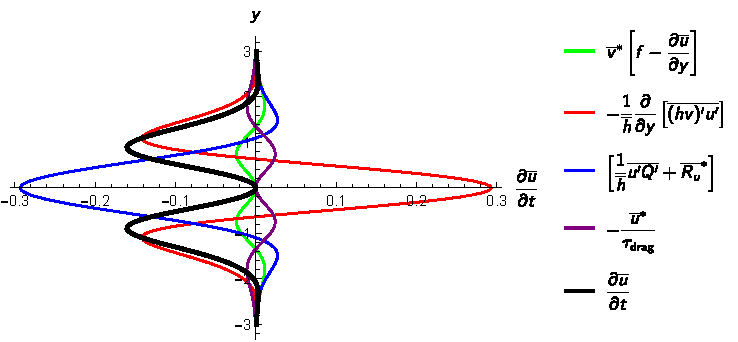
\includegraphics[width=0.85\textwidth]{figures/wave-mean-flow/matsuno-zonal-acceleration-terms.pdf}
  \caption{Acceleration terms.}
  \label{fig:matsuno-zonal-acceleration-terms}
\end{figure}


We can show that the acceleration must be zero at the equator for these forced shallow-water equations. Rewriting the zonal mean momentum equation in terms of the relative vorticity $\zeta$ \citep{thuburn1999zonalmean} \citep{showman2011superrotation}

\begin{equation}
  \frac { \partial \overline { u } } { \partial t } = \overline { v ^ { \prime } \zeta ^ { \prime } } + \overline { v } ( f + \overline { \zeta } ) - \frac { \overline { u } } { \tau _ { \mathrm { drag } } } + \overline { R _ { u } },
\end{equation}

we see that as $v=0$ at the equator (due to the symmetric forcing in $y$) $\frac { \partial \overline { u } } { \partial t } = 0$ at the equator also.

The fact that there is in the GCM simulations shows another process is affecting the zonal momentum at the equator. Note that this condition still applies to the same equations linearised about a zonal flow $\bar{U}(y)$ (Equation X).


% This also is necessary from the zonal momentum equation (the first line of Equation \ref{eqn:sw-eqns-1}). As the day-night forcing is symmetric about the equatorial, the meridional velocity $v$ must be zero at the equator. Also, the forcing $Q$ varies sinusoidally with $x$, so produces a sinusoidal response in $h$ along the equator, which will have a zonal mean of zero. Therefore, the zonal momentum equation requires that there is no zonal mean acceleration at the equator.


%SUBSECTION --
\subsection{Correction to Vertical Momentum Transport}

The forced shallow-water equations predict zero zonal acceleration at the equator. So, there must be another process at work at the equator producing the eastward zonal flow seen in GCM simulations.

\citet{showman2011superrotation} invoke a correction to the zonal momentum equation from \citet{shell2004superrotation}.

\begin{equation}\label{eqn:sw-eqns-R}
  \begin{gathered}
     \frac{\partial u}{\partial t} - \beta y v +\frac{\partial h}{\partial x} = R_{u} \\
      \frac{\partial v}{\partial t} + \beta y u + \frac{\partial h}{\partial y} = 0 \\
    \frac{\partial h}{\partial t} +c^{2}(\frac{\partial u}{\partial x} + \frac{\partial v}{\partial y}) = Q(x,y) \\
  \end{gathered}
\end{equation}

The correction $R_{u}$ represents the effect of exchanging zonal momentum between the active layer and the lower layer. On the day-side, air with zero angular momentum rises from the substellar point into the active layer, giving a zonal acceleration which opposes the local $u$ field. To conserve the vertically integrated local zonal momentum this acceleration is $R_{u} - \frac { Q u } { h }$ \citep{showman2011superrotation}. On the night-side, air leaves the active layer which does not affect the local angular momentum, so $R_{u}=0$.

\begin{equation}
   R _{u}  = \left\{ \begin{array} { l l } { - \frac { Q u } { h } , } & { Q > 0 } \\ { 0 , } & { Q < 0 } \end{array} \right
\end{equation}

This modifies the zonal mean momentum equation to:

\begin{equation}\label{eqn:zonal-mean-mom-with-R}
  \frac { \partial \overline { u } } { \partial t } = \underbrace { \overline { v } ^ { * } \left[ f - \frac { \partial \overline { u } } { \partial y } \right] } _ { I } \underbrace { - \frac { 1 } { \overline { h } } \frac { \partial } { \partial y } \left[ \overline { ( h v ) ^ { \prime } u ^ { \prime } } \right] } _ { I I } + \underbrace { \left[ \frac { 1 } { \overline { h } } \overline { u ^ { \prime } Q ^ { \prime } } + \overline { R _ { u } } ^ { * } \right] } _ { I I I } \underbrace { - \frac { \overline { u } ^ { * } } { \tau _ { \mathrm { drag } } } } _ { I V } - \frac { 1 } { \overline { h } } \frac { \partial \left( \overline { h ^ { \prime } u ^ { \prime } } \right) } { \partial t }
\end{equation}

Figure \ref{fig:matsuno-zonal-acceleration-terms-with-R} shows the terms Equation \ref{eqn:zonal-mean-mom-with-R}. In comparison to Figure \ref{fig:matsuno-zonal-acceleration-terms}, there is now a zonal acceleration at the equator.

\begin{figure}
  \centering
  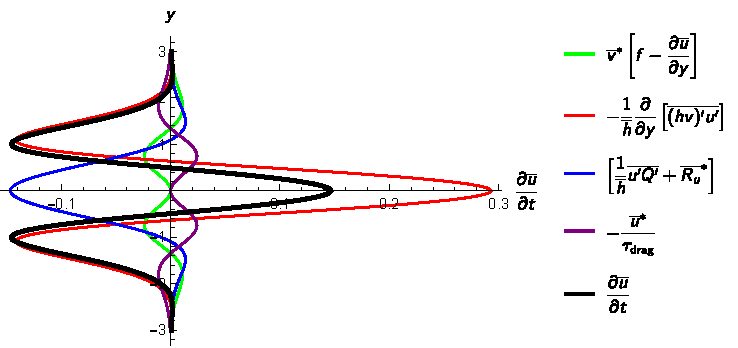
\includegraphics[width=0.85\textwidth]{figures/wave-mean-flow/matsuno-zonal-acceleration-terms-with-R.pdf}
  \caption{Acceleration terms with R.}
  \label{fig:matsuno-zonal-acceleration-terms-with-R}
\end{figure}

Rewriting the zonal mean momentum equation in terms of the relative vorticity again shows that there is now a non-zero acceleration at the equator due to $R_{u}$:

\begin{equation}
  \frac { \partial \overline { u } } { \partial t } = \overline { v ^ { \prime } \zeta ^ { \prime } } + \overline { v } ( f + \overline { \zeta } ) - \frac { \overline { u } } { \tau _ { \mathrm { drag } } } + \overline { R _ { u } },
\end{equation}

This explains the equatorial superrotation on tidally locked planets. But, it does not explain why momentum-conserving retrograde westward flow predicted by this shallow-water model in the mid-latitudes, does not appear in the GCM simulations, which instead have an atmosphere superrotating at most latitudes. In Chapter XX I will discuss this.

%SUBSECTION --
\subsection{Equilibrium Equatorial Flow}

This provides an estimate of the equilibrium zonal flow speed on the equator, which will occur when $\frac { \partial \overline { u } } { \partial t }=0$:

\begin{equation}
  \frac { \overline { u } } { \tau _ { \mathrm { drag } } } = \overline { R _ { u } },
\end{equation}

As the zonal flow $\overline { u }$ increases, the drag term $\frac { \overline { u } } { \tau _ { \mathrm { drag } } }$ will increase until it balances the acceleration due to vertical momentum transport $\overline { R _ { u } }$.

The acceleration due to vertical momentum transport $\overline { R _ { u } }$ will also decrease as the zonal flow $\overline { u }$ increases, so even if $\tau_{drag}$ is very large and  $\frac { \overline { u } } { \tau _ { \mathrm { drag } } }$ is negligible, $\overline { R _ { u } }$ will eventually become zero for large enough zonal flow, and the acceleration will become zero. \citet{showman2011superrotation} suggest that $\overline { R _ { u } }$ simply gets smaller as the zonal mean $\overline{u}$ gets larger. Later, I will add the fact that the forced response is Doppler-shifted eastwards, changing the part of the eddy response that is on the day-side and contributes to $\overline { R _ { u } }$.

In addition, I will show how this eastward shift decreases term II in Equation \ref{eqn:zonal-mean-mom-with-R} by shifting the different wave components closer together. This further decreases the equatorial acceleration as the zonal flow increases, making it reach an equilibrium sooner.


%SUBSECTION --
\subsection{Horizontal Momentum Transport from Stationary Waves}

It is helpful to now consider the terms in Equation \ref{eqn:zonal-mean-mom} in more detail.

Term II in Equation \ref{eqn:zonal-mean-mom} is the horizontal momentum transport. The sign of Term II depends on the

But, it is cancelled out by the vertical momentum transport.


%SUBSECTION --
\subsection{Horizontal Momentum Transport from Transient Waves}



%SECTION CONCLUSIONS

%%%%%%%%%%%%%%%%%%%%%%%%%%%%%%%%%%%%


%SECTION 3 -- SHEAR FLOW ON BETA-PLANE AND SPHERICAL
\section{Wave Interactions with Shear Flow on the Beta-Plane}\label{sec:shear-flow-beta-plane}

In this section, I discuss the main result of this chapter -- the forced response of the shallow-water equations linearized around a zonally uniform shear flow $\bar{U}(y)$ and height $\bar{H}(y)$. I will show that the form of this forced response matches the results of GCM simulations, and suggest that the equatorial jet is therefore vital in controlling the global temperature structure and circulation pattern.

The background flow $\bar{U}(y)$ and height $\bar{H}(y)$ satisfy the second line of Equation \ref{eqn:sw-eqns-R}, so are geostrophically balanced with $\bar{H}_{y}(y)=-y\bar{U}(y)$. For our Gaussian jet $\bar{U}(y)=U_{0}e^{-y^{2}/2}$, the height perturbation is therefore $\bar{H}(y)=U_{0}e^{-y^{2}/2}$ \citep{hammond2018wavemean}.

For the tests in this chapter, I use a forcing magnitude $Q_{0}=1$ and equal radiative and dynamical damping rates $\alpha_{rad}=\alpha_{dyn} = 0.2$ \citep{matsuno1966quasi}. I will show the effect of varying these damping rates in Section X.

The tests in this section will show the effect of a zonal flow with a maximum non-dimensional speed between 0 and 1, as this is the speed required for a significant zonal shift of the forced response, as discussed in Section X.

The value of $Q_{0}=1$ in the forcing $Q(y)=Q_{0}\sin(x)e^{-y^{2}/2}$ was chosen to produce a comparable perturbation to that from the imposed equatorial jet, and to be consistent with \citet{matsuno1966quasi} and \citet{showman2011superrotation}. Later in Section XX I will use a a different (and more realistic) forcing value, to satisfy this condition in a spherical geometry with a different balance between jet velocity and jet height.

%For the forced response to be similar to the results of GCM simulations like those in Figure \ref{fig:example-gcm-results}, the strength of the height perturbation $\overline{H}(y)=-y\bar{U}(y)$ from the jet $\overline{U}(y)$ must be comparable to the strength of the height perturbation $\alpha_{rad}Q(y)$ from the forcing $Q(y)$.

Linearised around the background flow $\bar{U}(y)$ and height $\bar{H}(y)$, the shallow-water equations in Section X become:

\begin{equation}\label{eqn:shear-sw-equations}
    \begin{gathered}
      \frac{\partial u}{\partial t} +  \alpha_{dyn} u + \frac{\partial \bar{U}(y)u}{\partial x} +(\frac{\partial \bar{U}(y)}{\partial y} - y)v + \frac{\partial h}{\partial x} = 0 \\
      \frac{\partial v}{\partial t} +  \alpha_{dyn} v + \frac{\partial \bar{U}(y)v}{\partial x} + y u + \frac{\partial h}{\partial y} = 0 \\
      \frac{\partial \bar{H}' u}{\partial x} + \bar{H}'\frac{\partial v}{\partial y} - y\bar{U}(y) v +\frac{\partial h}{\partial t} +  \alpha_{rad} h + \frac{\partial \bar{U}(y) h}{\partial x} = Q(y)\\
        \bar{H}' = 1+\bar{H}(y)
    \end{gathered}
\end{equation}


To consider the free modes of this system, we set $Q(y)=0$ and $\partial /\partial t = -i \omega$, and write $u,v,h$ in the form form $A(y) e^{i(k_{x}x - \omega t)}$:


  \begin{equation}\label{eqn:free-sw-shear}
    \begin{gathered}
      \begin{pmatrix}
      \alpha_{dyn} + i k_{x}\bar{U}(y) & \frac{\partial\bar{U}(y)}{\partial y}-y & i k_{x} \\
      y & \alpha_{dyn} + i k_{x}\bar{U}(y) & \frac{\partial}{\partial y} \\
      i k_{x} \bar{H}' & -y \bar{U}(y) + \bar{H}' \frac{\partial}{\partial y} & \alpha_{rad} + k_{x}\bar{U}(y)
      \end{pmatrix}
      \begin{pmatrix}
      u \\
      v \\
      h
      \end{pmatrix}
      =
      i \omega
      \begin{pmatrix}
      u \\
      v \\
      h
      \end{pmatrix} \\
        \bar{H}' = 1+\bar{H}(y)
    \end{gathered}
  \end{equation}

To find the stationary response to steady forcing, we set we set $Q(y)=Q_{0}e^{-y^{2}/2}$ \citep{matsuno1966quasi} and $\partial / \partial t = 0 $, giving the linear system of equations:


\begin{equation}\label{eqn:forced-sw-shear}
  \begin{gathered}
    \begin{pmatrix}
    \alpha_{dyn} + i k_{x}\bar{U}(y) & \frac{\partial\bar{U}(y)}{\partial y}-y & i k_{x} \\
    y & \alpha_{dyn} + i k_{x}\bar{U}(y) & \frac{\partial}{\partial y} \\
    i k_{x}\bar{H}' & -y \bar{U}(y) + \bar{H}' \frac{\partial}{\partial y} & \alpha_{rad} + k_{x}\bar{U}(y)
    \end{pmatrix}
    \begin{pmatrix}
    u \\
    v \\
    h
    \end{pmatrix}
    =
    \begin{pmatrix}
    0 \\
    0 \\
    Q(y)
    \end{pmatrix} \\
      \bar{H}' = 1+\bar{H}(y)
  \end{gathered}
\end{equation}

I solved both the free and forced systems of equations using the method in Appendix X, expanding the solutions in terms of the parabolic cylinder functions. This method identifies the exact free and forced solutions in the case where $\overline{U}(y)=0$, and finds the solutions with non-zero $\overline{U}(y)$ to better than 1 part in 10,000 when 30 basis modes are used in the calculation. In Appendix X, I show the accuracy of this method in more detail.

Finally, it is worth noting that I have considered the perturbations in the forced system to apply to a single shallow-water layer of height $H_{0}$, non-dimensionalised to unity. Technically, the vertically varying heating profile in a planetary atmosphere excites a continuum of vertical modes, each defining a shallow-water system of different $H_{0}$. However, \citet{tsai2014three} showed that in this forced shallow-water system, almost all of the energy is confined to the lowest-order vertical mode, making the assumption that a real atmosphere is described well by a single shallow-water layer reasonable.

 % Appendix \ref{sec:app-beta} shows the accuracy of this method, demonstrating that the pseudo-spectral method identifies the exact solution in the case with no background jet, and that the solution with a background flow changes by less than 1 part in 10,000 for any modes past $n=30$. The pseudo-spectral method finds $N_{m}$ solutions (the number of modes used in the calculation) for the eigenvalue equation governing the free modes. Many of these are spurious, but we can distinguish them from the physical modes by inspecting their eigenvalues. The pseudo-spectral method only produces a single solution for the forced linear system, which is simpler to interpret.



%SUBSECTION --
\subsection{Free Modes}

\begin{figure}
  \centering
  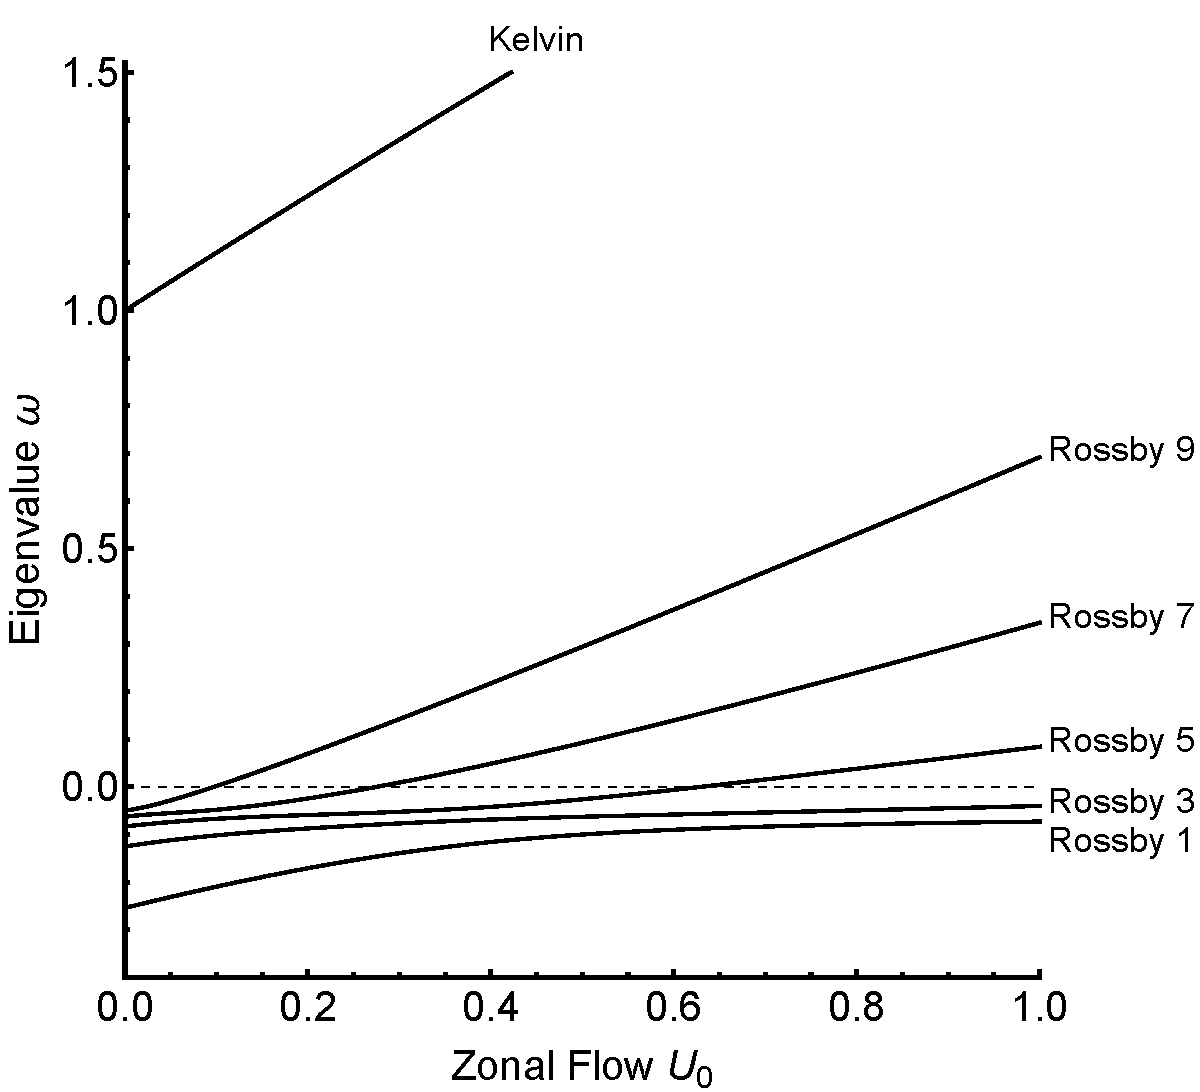
\includegraphics[width=0.6\textwidth]{figures/wave-mean-flow/shear-flow-eval-shift.pdf}
  \caption{Eigenvalue shift.}
  \label{fig:shear-flow-eval-shift}
\end{figure}

\begin{figure}
  \begin{subfigure}[b]{0.33\textwidth}
    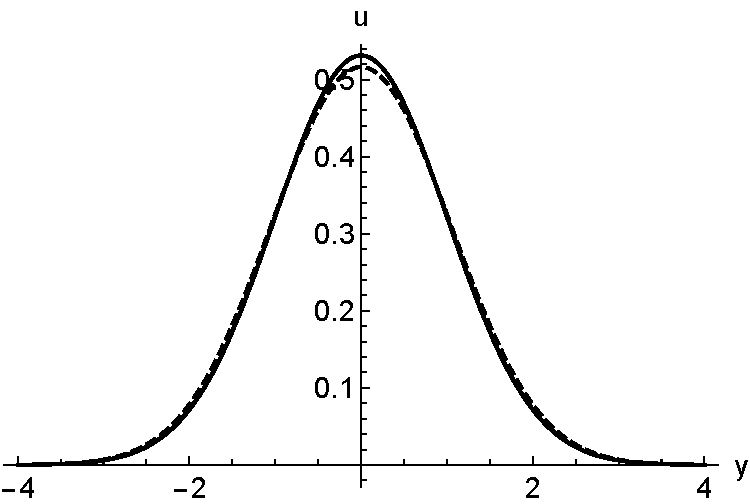
\includegraphics[width=\textwidth]{figures/wave-mean-flow/free-u-shear-kelvin.pdf}
    \caption{Zonal velocity.}
    \label{fig:free-u-shear-kelvin}
  \end{subfigure}
  %
  \begin{subfigure}[b]{0.33\textwidth}
    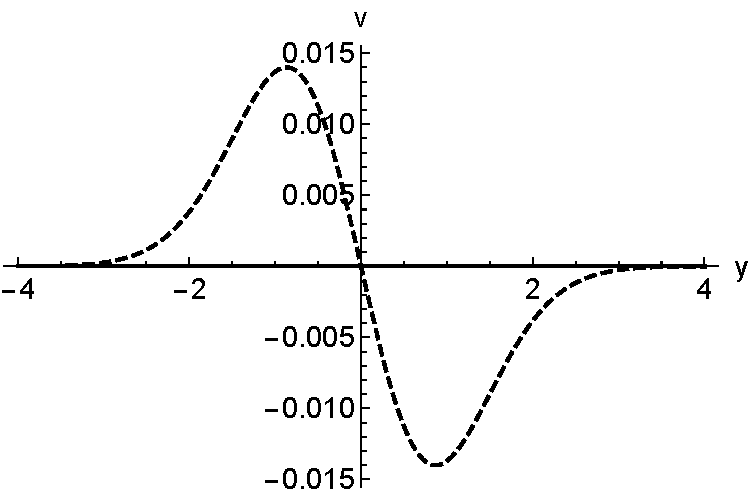
\includegraphics[width=\textwidth]{figures/wave-mean-flow/free-v-shear-kelvin.pdf}
    \caption{Meridional velocity.}
    \label{fig:free-v-shear-kelvin}
  \end{subfigure}
  %
  \begin{subfigure}[b]{0.33\textwidth}
    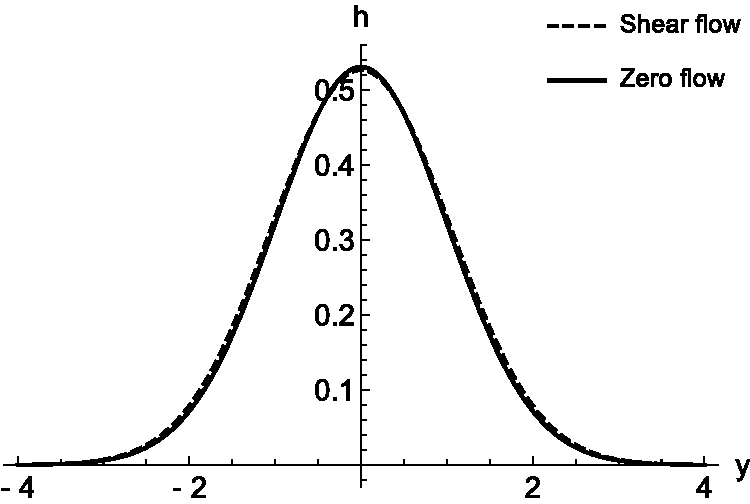
\includegraphics[width=\textwidth]{figures/wave-mean-flow/free-h-shear-kelvin.pdf}
    \caption{Height.}
    \label{fig:free-h-shear-kelvin}
  \end{subfigure}
  %
  \caption{The meridional structure of the free Kelvin mode.}
  \label{fig:free-shear-meridional-kelvin}
\end{figure}

\begin{figure}
  \begin{subfigure}[b]{0.33\textwidth}
    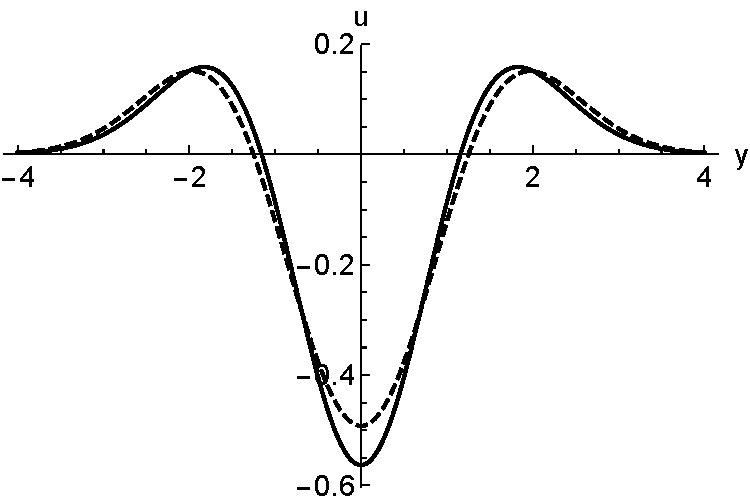
\includegraphics[width=\textwidth]{figures/wave-mean-flow/free-u-shear.pdf}
    \caption{Zonal velocity.}
    \label{fig:free-u-shear}
  \end{subfigure}
  %
  \begin{subfigure}[b]{0.33\textwidth}
    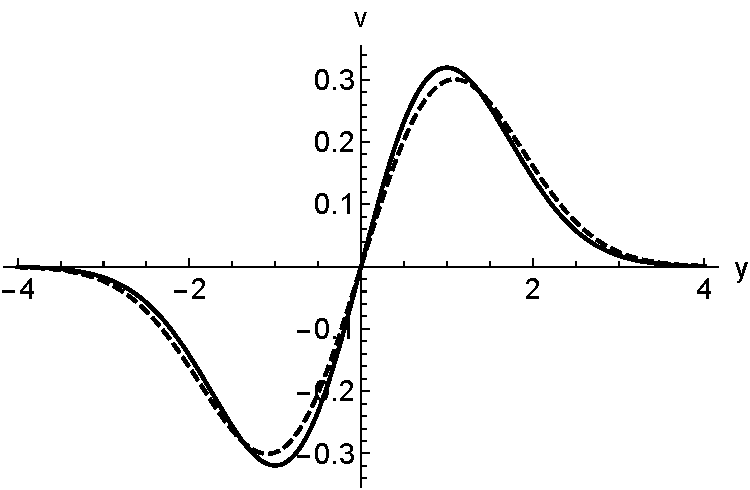
\includegraphics[width=\textwidth]{figures/wave-mean-flow/free-v-shear.pdf}
    \caption{Meridional velocity.}
    \label{fig:free-v-shear}
  \end{subfigure}
  %
  \begin{subfigure}[b]{0.33\textwidth}
    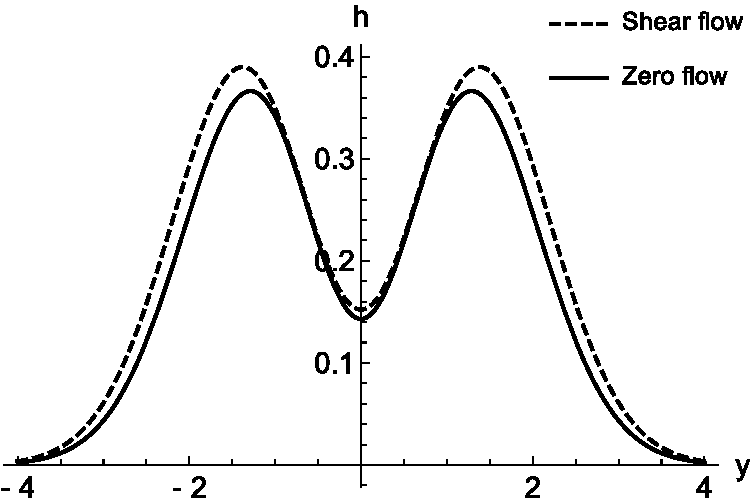
\includegraphics[width=\textwidth]{figures/wave-mean-flow/free-h-shear.pdf}
    \caption{Height.}
    \label{fig:free-h-shear}
  \end{subfigure}
  %
  \caption{The meridional structure of the free Rossby mode \citep{hammond2018wavemean}.}
  \label{fig:free-shear-meridional}
\end{figure}


%%%%%%%%

In this section, I will discuss the effect of a background shear flow on the free modes of the shallow-water equations. This will be useful to understand the effect of the background flow on the forced response, in the next section.

In Section \ref{sec:shallow-water}, I showed how the response to a forcing can be written as a sum of the free modes of the system. It is not possible to write down an exact solution like this when the system is linearised about a background flow $\overline{U}(y)$ and $\overline{H}(y)$, but it is still useful to interpret the resulting solution in terms of the fundamental free modes.

I will write the free solutions to shallow-water equations as a complex function of latitude $A(y)$. and the forced solutions as functions of both latitude and longitude in the form $A(y) e^{i \delta(y) x}$. This phase $\delta(y)$ determines the longitudinal structure of the forced response, and is equivalent to the phase shift $(\omega_{m} - k_{x} \bar{U})$ derived for a uniform flow in Section XX.

We can still consider the response to forcing as a sum of the free modes of the system, as in Section X. Now the equations are linearised about a shear flow $\overline{U}(y)$ and $\overline{H}(y)$, the free modes have a different latitudinal structure $u(y),v(y),h(y)$ and have different eigenvalues $\omega_{m}$ (so will have different longitudinal position in the forced response).

I found the free modes of the shallow-water system defined by Equation \ref{eqn:free-sw-shear} using the method in Appendix X. Figure \ref{fig:shear-flow-eval-shift} shows the real parts of the eigenvalues of the free Kelvin mode and the symmetric free Rossby modes of Equation \ref{eqn:free-sw-shear}, for a background flow $\bar{U}(y)=U_{0}e^{-y^{2}/2}$ with a variable magnitude $U_{0}$ \citep{hammond2018wavemean}. I plot these modes as they are the lowest-order (so largest magnitude) modes excited by the symmetric, stationary forcing.

The value and sign of these eigenvalues determine the position of the free mode in the forced response, similar to Equation X in Section X. Note that an exact forced solution in terms of a series free modes is now not possible as the flow is not uniform, but it is still very useful to interpret the forced response in this way.

As the magnitude $U_{0}$ of the equatorial jet $\overline{U}(y)$ increases, all of the eigenvalues of the free modes become more positive, corresponding to an eastward shift in their position in the forced response (as in Equation X in Section X). The Kelvin mode already has a positive eigenvalue for $U_{0}=0$ (hence its position in Figure \ref{fig:motivate-showman}), and this becomes larger as $U_{0}$ increases, so the Kelvin mode becomes further east in the forced response. The maximum shift of the modes is to $+90\degr$ east of the substellar point (as in Equation X), no matter how large the eigenvalue becomes. This shift leads to the large eastward equatorial hot-spot shift that will be seen later.

The Rossby modes are a little more complicated. \citet{tsai2014three} shows that in a uniform background flow, the $n=1$ Rossby mode is shifted eastwards towards $+90\degr$, producing a hot-spot shift (reproduced in Figure \ref{fig:motivate-tsai}). In fact, Figure \ref{fig:shear-flow-eval-shift} shows that in this non-uniform flow $\bar{U}(y)$, the $n=1$ Rossby mode eigenvalue becomes less negative but does not become positive for $U_{0}=1.0$. This means that in the forced response it is shifted eastwards, but not far enough to pass the substellar point.

The higher order Rossby modes are shifted by the flow $\overline{U}(y)$, as shown by their positive eigenvalues for high enough flow speed $U_{0}$. However, the higher the order of a mode, the weaker its contribution to the forced response \citep{matsuno1966quasi}. The $n=3$ and $n=5$ symmetric Rossby modes are still important to the forced response, but any modes beyond this are less important.

%%%%%%%%




\textbf{That is not to say that the $n=1$ mode is never responsible for the hot-spot shift -- later, we will show that in a spherical geometry the $n=1$ mode shifts close to $+90\degr$ eastwards. It is also possible in the beta-plane system for different input parameters (flow speed, damping rates) to shift the $n=1$ Rossby mode past the substellar point. But, our free mode expansion has shown that the $n=1$ Rossby mode is not the only important mode, and that the higher-order modes are also important to the forced response.}

For zero damping, half of these eigenvalues will have positive imaginary parts, and the modes corresponding to them will grow exponentially. Non-zero damping decreases the imaginary part of all the modes, so will make some or all of these modes stable. In general, the free linear system in Equation \ref{eqn:free-sw-shear} will have some unstable modes unless the damping is very large. These unstable modes are similar to those discussed by \citet{wang2014instability}, who show how similar modes can produce superrotation even on a planet without a permanent day-night heating difference.

These unstable modes technically make the linear forced wave problem ill-posed, since the result of any linear initial value problem will be eventually dominated by the most rapidly growing modes rather than the stationary response. Later comparison with nonlinear GCM simulations in Section \ref{sec:gcm-results} will show that the forced response still has considerable explanatory power. This may be because in reality the unstable modes equilibrate due to damping or nonlinear effects, at a sufficiently low amplitude that they take the form of mobile waves propagating across the forced stationary pattern without significantly disrupting its basic structure. Future work should investigate the exact nature of these instabilities, and the effect of damping and shear flow on their growth rates.

The shear flow also affects the latitudinal structure $A(y)$ of the modes. The lowest-order free solutions of Equation \ref{eqn:free-sw-shear} (the Kelvin and Rossby modes), plotted in Figure \ref{fig:free-shear-meridional} and \ref{fig:free-shear-meridional-kelvin}, resemble the free solutions with zero shear flow \citep{matsuno1966quasi}, with their latitudinal structure slightly changed \textbf{by a weak shear flow $\bar{U}=0.1 e^{-y^{2}/2}$}. The shear flow perturbs the solutions by adding higher order meridional structure.  For example, the meridional wind of the Rossby wave in Figure \ref{fig:free-shear-meridional} resembles the $n=1$ \textbf{parabolic cylinder function} added to the $n=3$ function (see Figure \ref{fig:hermite-functions} in Appendix \ref{sec:app-ps-method}). \textbf{\citet{boyd1978shearI} discusses how a shear flow affects the meridional structure of these modes in more detail.}



%SUBSECTION --
\subsection{Forced Solutions}

Figure X shows the forced solution in shear flow.


\begin{figure}
  \centering
  \begin{subfigure}[b]{0.49\textwidth}
    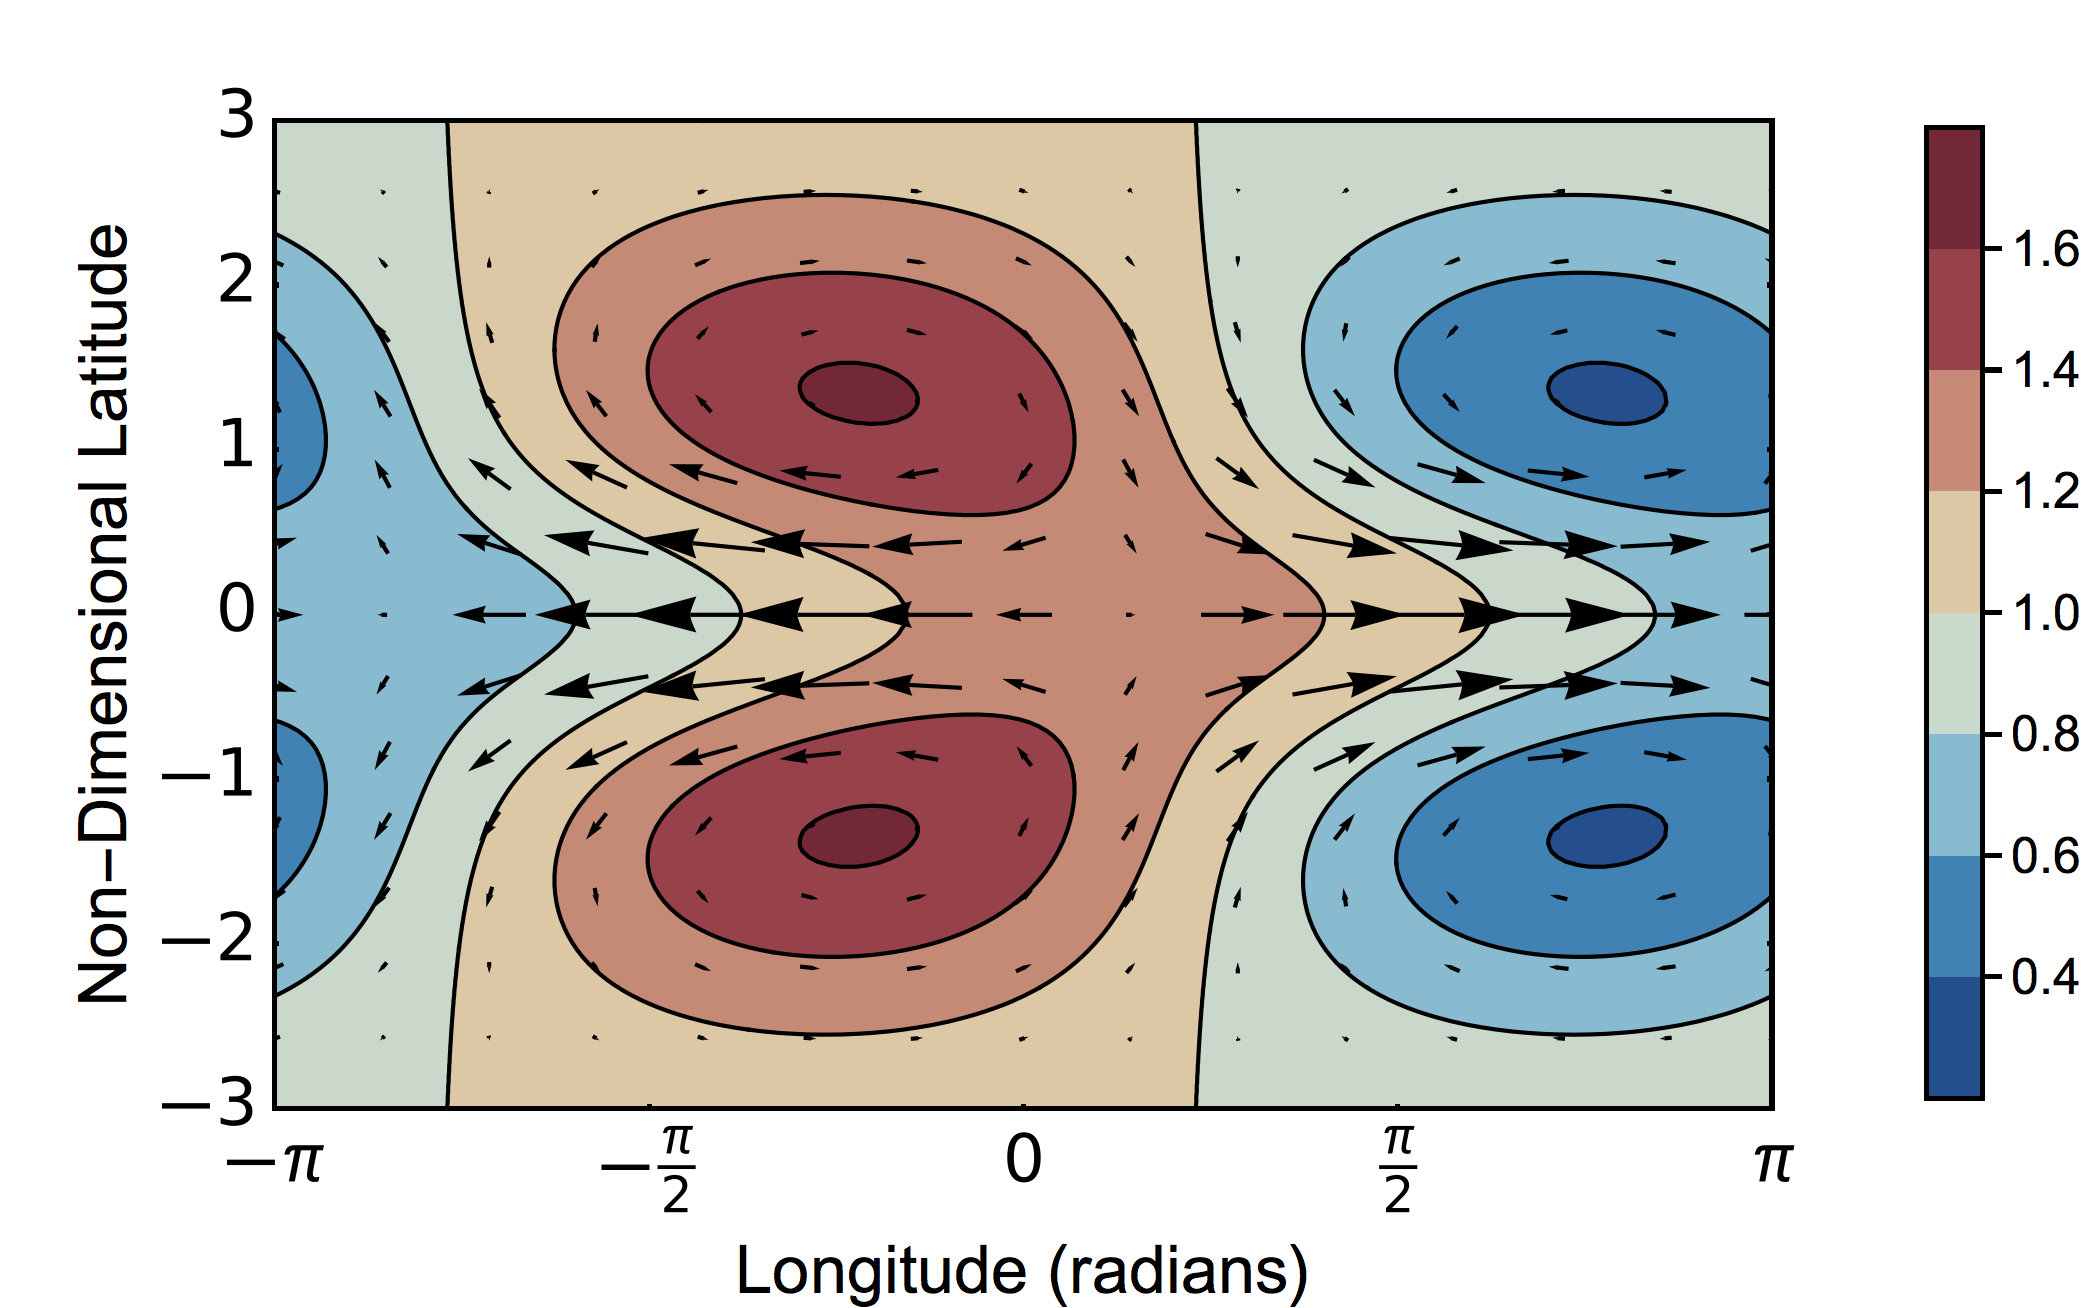
\includegraphics[width=\textwidth]{figures/wave-mean-flow/ps-no-flow.png}
    \caption{Zero Flow.}
    \label{fig:ps-no-flow}
  \end{subfigure}
  %
  \begin{subfigure}[b]{0.49\textwidth}
    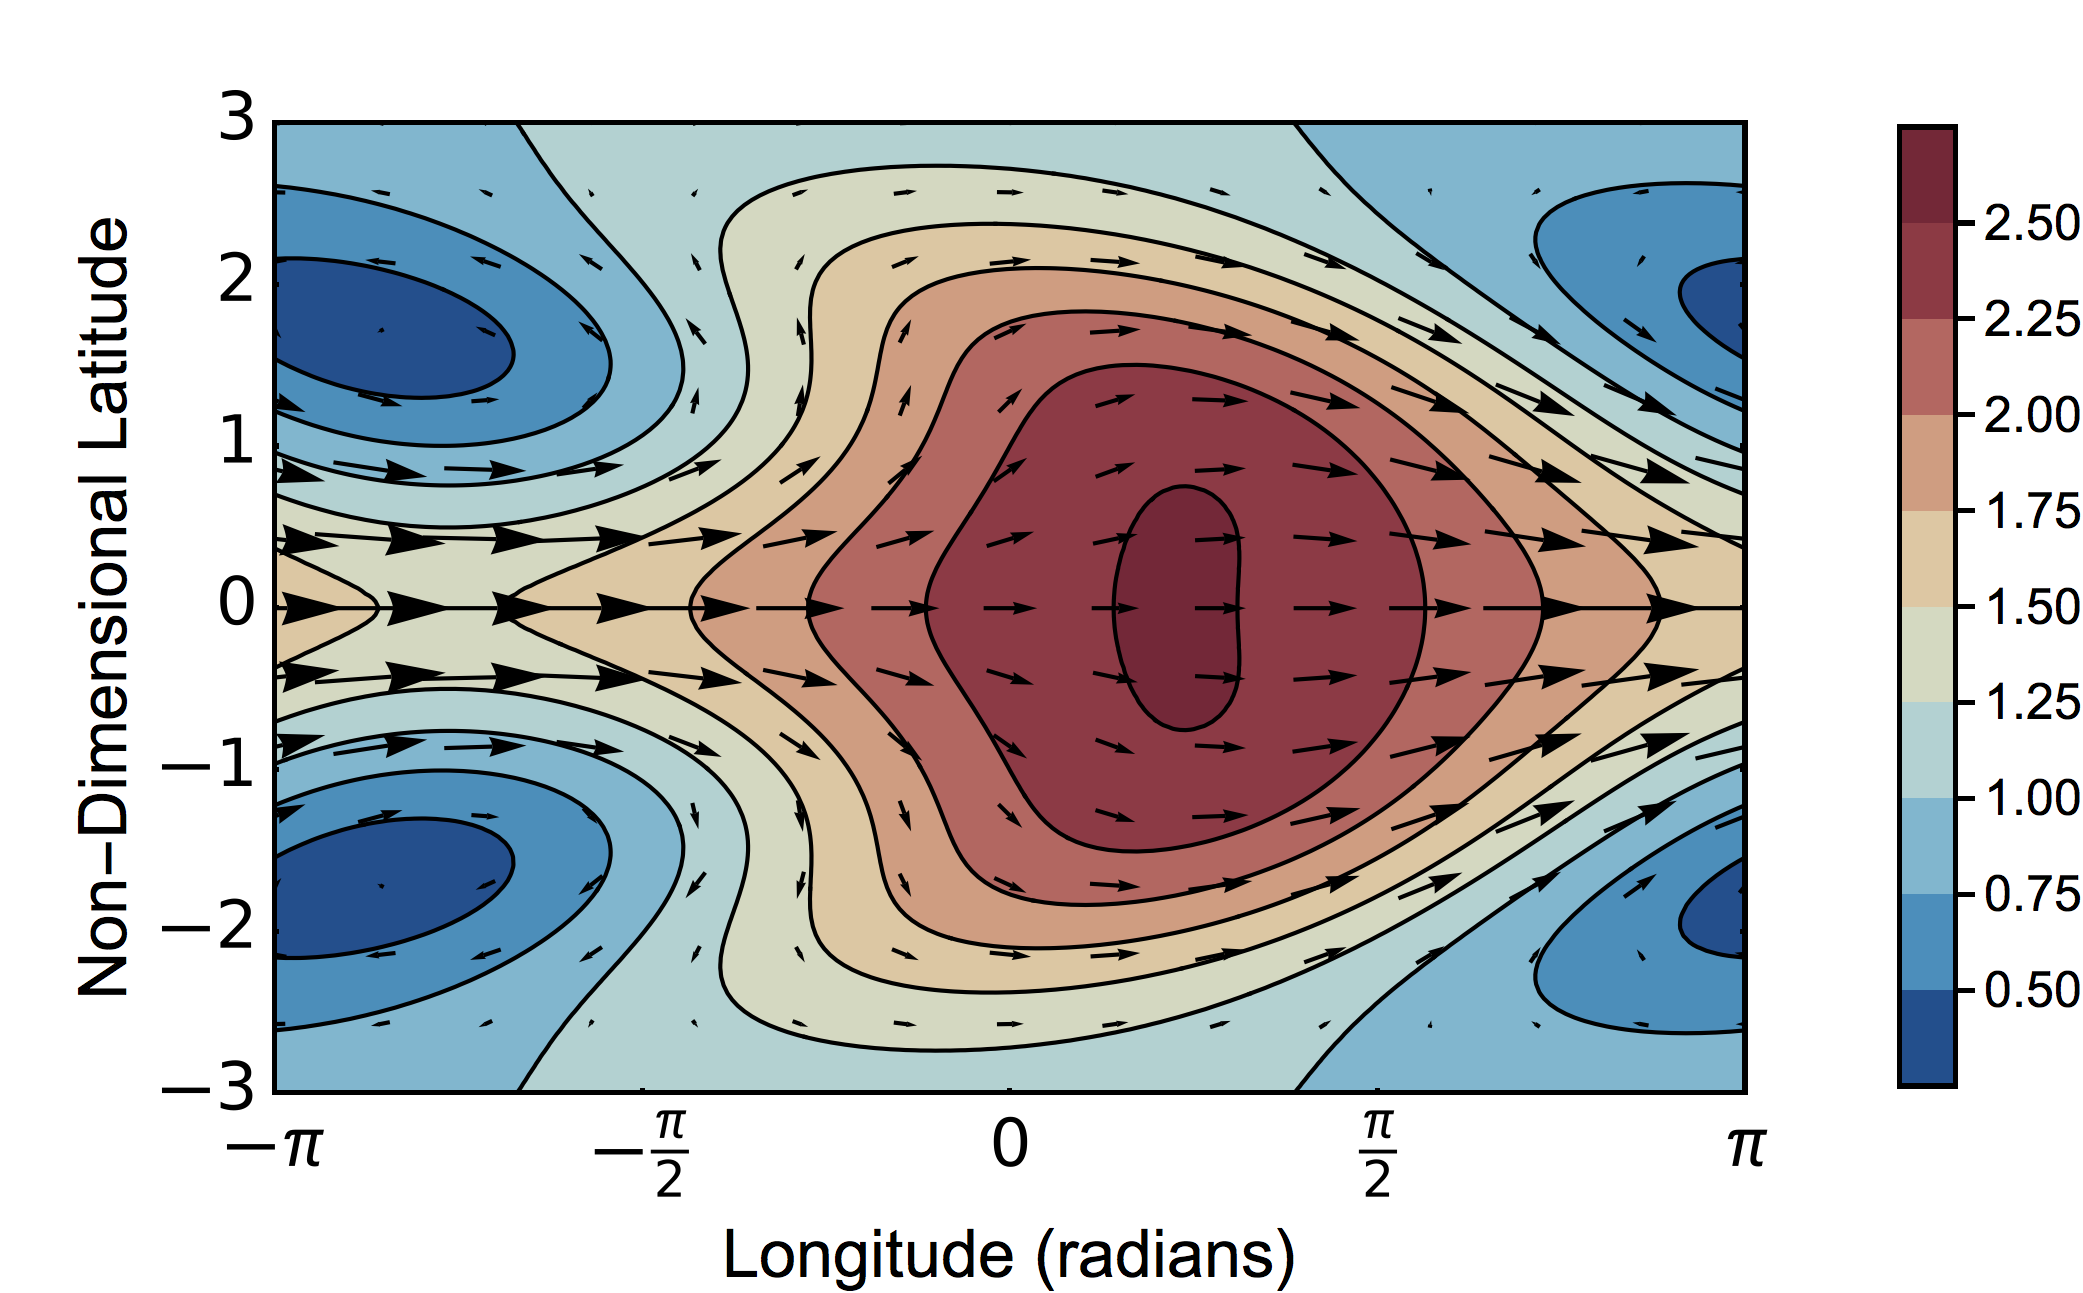
\includegraphics[width=\textwidth]{figures/wave-mean-flow/ps-shear-flow.png}
    \caption{Shear Flow.}
    \label{fig:ps-shear-flow}
  \end{subfigure}
  \caption{Zero Flow and Shear Flow.}
  \label{fig:ps-flow}
\end{figure}


%SUBSECTION --
\subsection{Equilibrium Circulation}

\begin{figure}
  \centering
  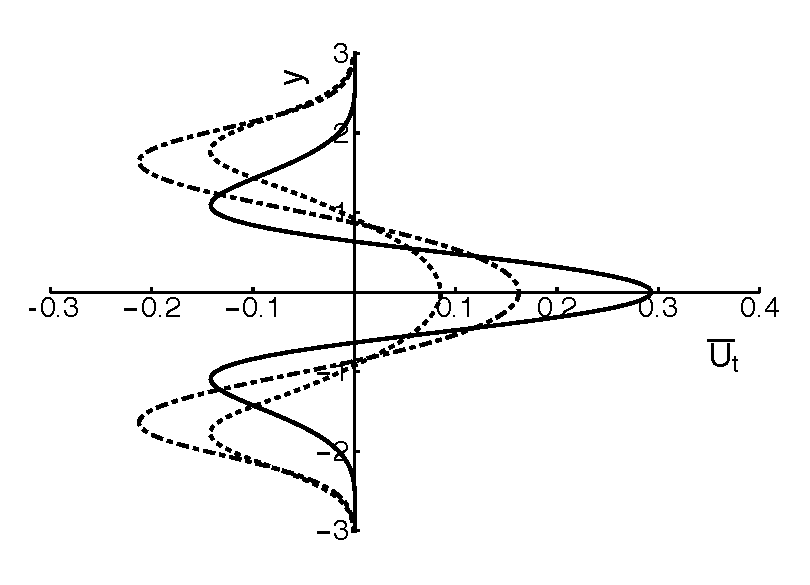
\includegraphics[width=0.6\textwidth]{figures/wave-mean-flow/accn-vs-u.pdf}
  \caption{Acceleration versus speed}
  \label{fig:accn-vs-u}
\end{figure}

The equatorial superrotation reaches a steady equilibrium when the zonal acceleration is zero.

As discussed in Section \ref{sec:zonal-acceleration}, the equatorial acceleration decreases as the zonal flow increases, reaching an equilibrium when the acceleration is zero.

%SUBSECTION --
\subsection{Damping}


\begin{figure}
  \centering
  \begin{subfigure}[b]{0.49\textwidth}
    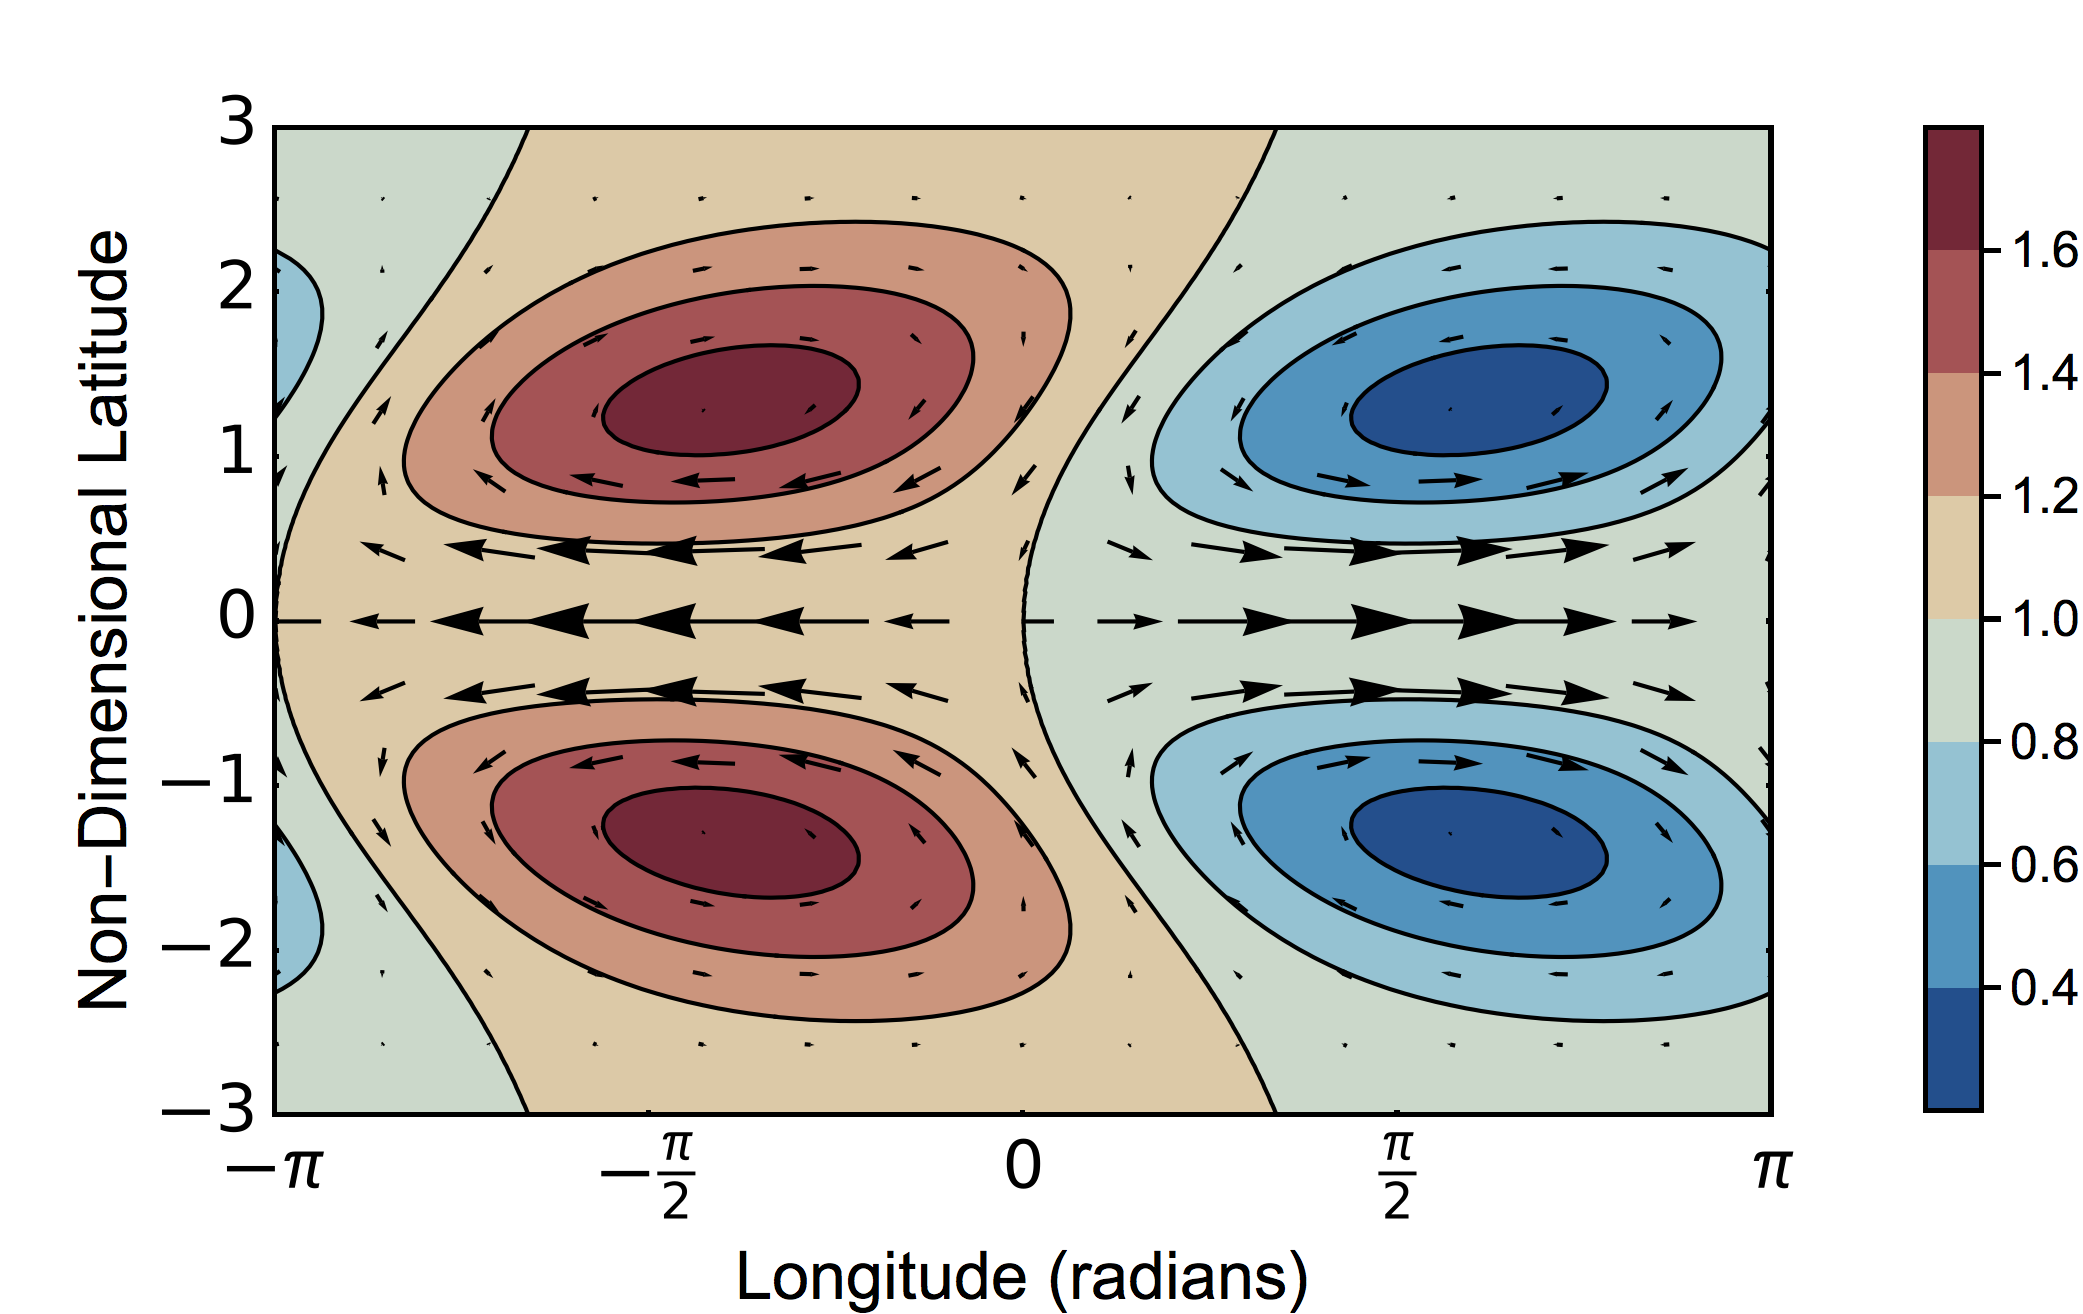
\includegraphics[width=\textwidth]{figures/wave-mean-flow/zero-alpha-dyn-zero-flow.png}
    \caption{Zero Flow.}
    \label{fig:zero-alpha-dyn-zero-flow}
  \end{subfigure}
  %
  \begin{subfigure}[b]{0.49\textwidth}
    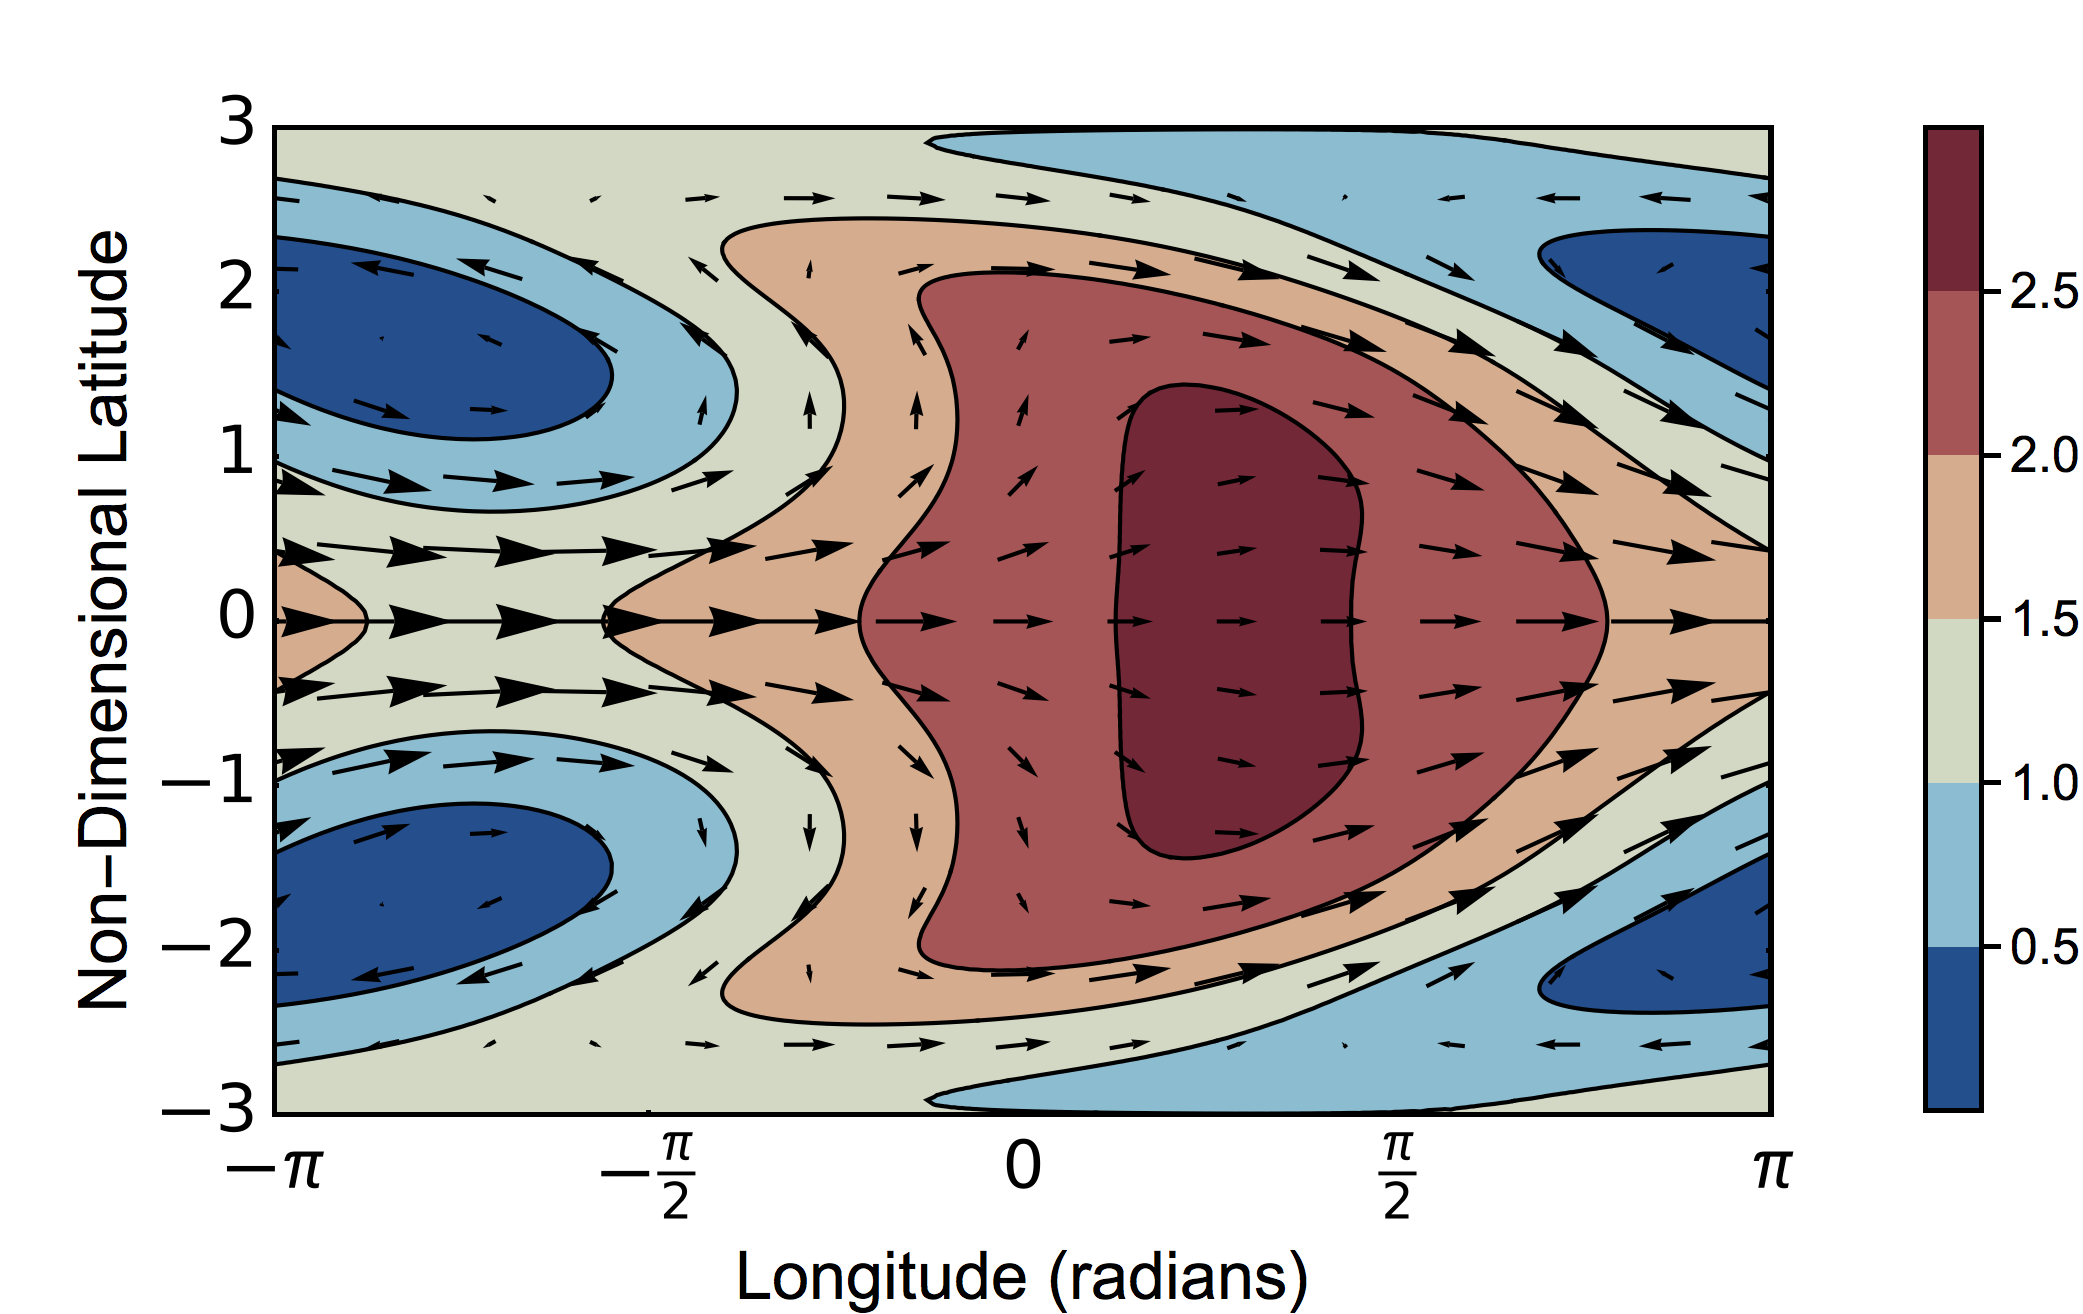
\includegraphics[width=\textwidth]{figures/wave-mean-flow/zero-alpha-dyn-1-flow.png}
    \caption{Shear Flow.}
    \label{fig:zero-alpha-dyn-1-flow}
  \end{subfigure}
  \caption{Zero Flow and Shear Flow.}
  \label{fig:zero-alpha-dyn-flow}
\end{figure}


Figure X shows the effect of different damping rates.

%SUBSECTION --
\subsection{Hot-Spot Shift}


\begin{figure}
  \centering
  \begin{subfigure}[b]{0.24\textwidth}
    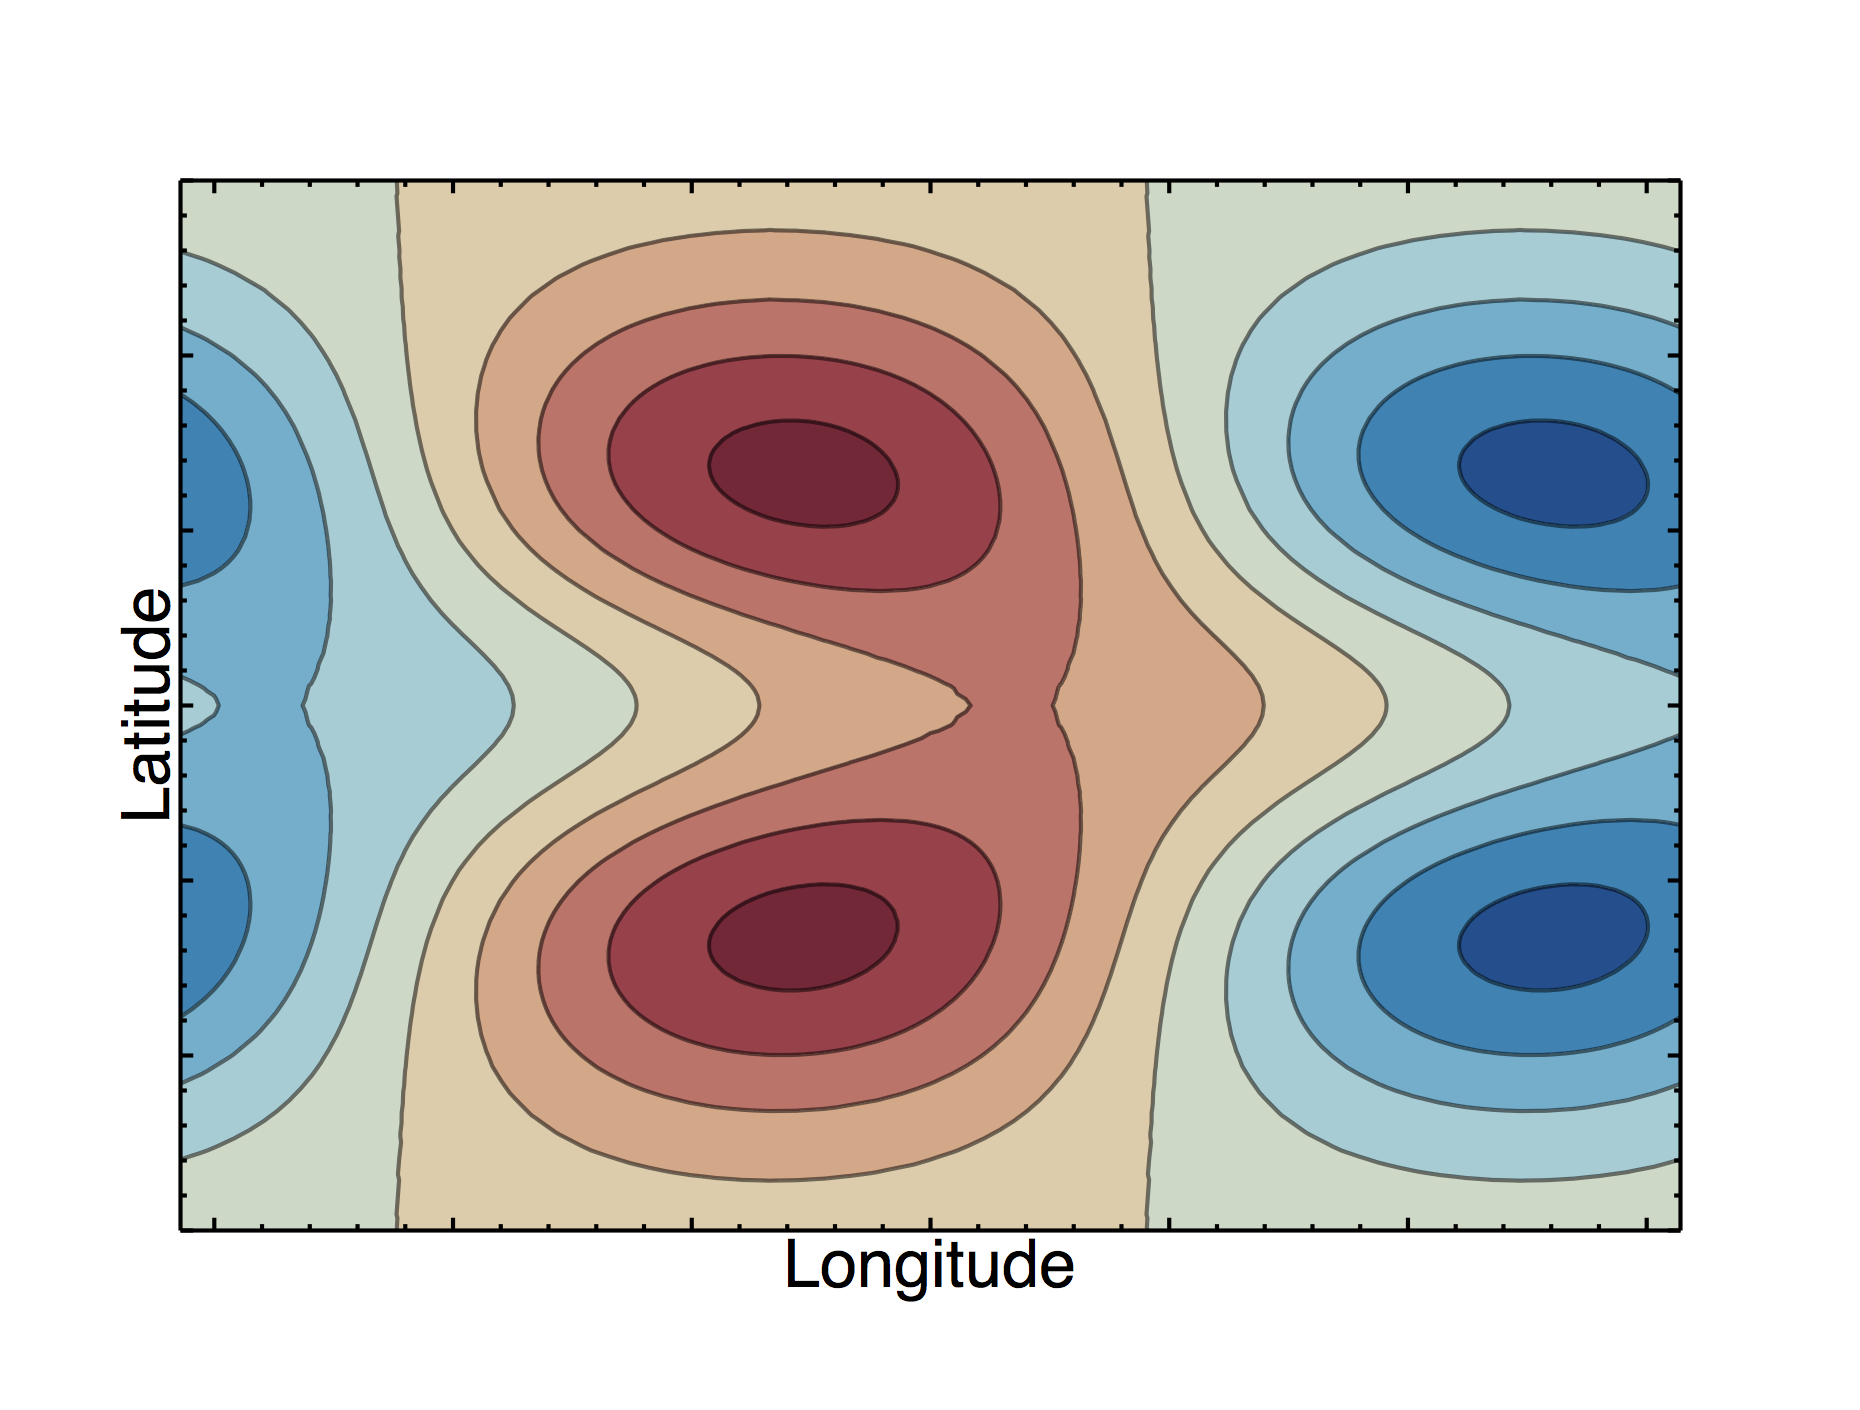
\includegraphics[width=\textwidth]{figures/wave-mean-flow/expl-non-shifted-matsuno.png}
    \caption{Zero Flow.}
    \label{fig:expl-non-shifted-matsuno}
  \end{subfigure}
  %
  \begin{subfigure}[b]{0.24\textwidth}
    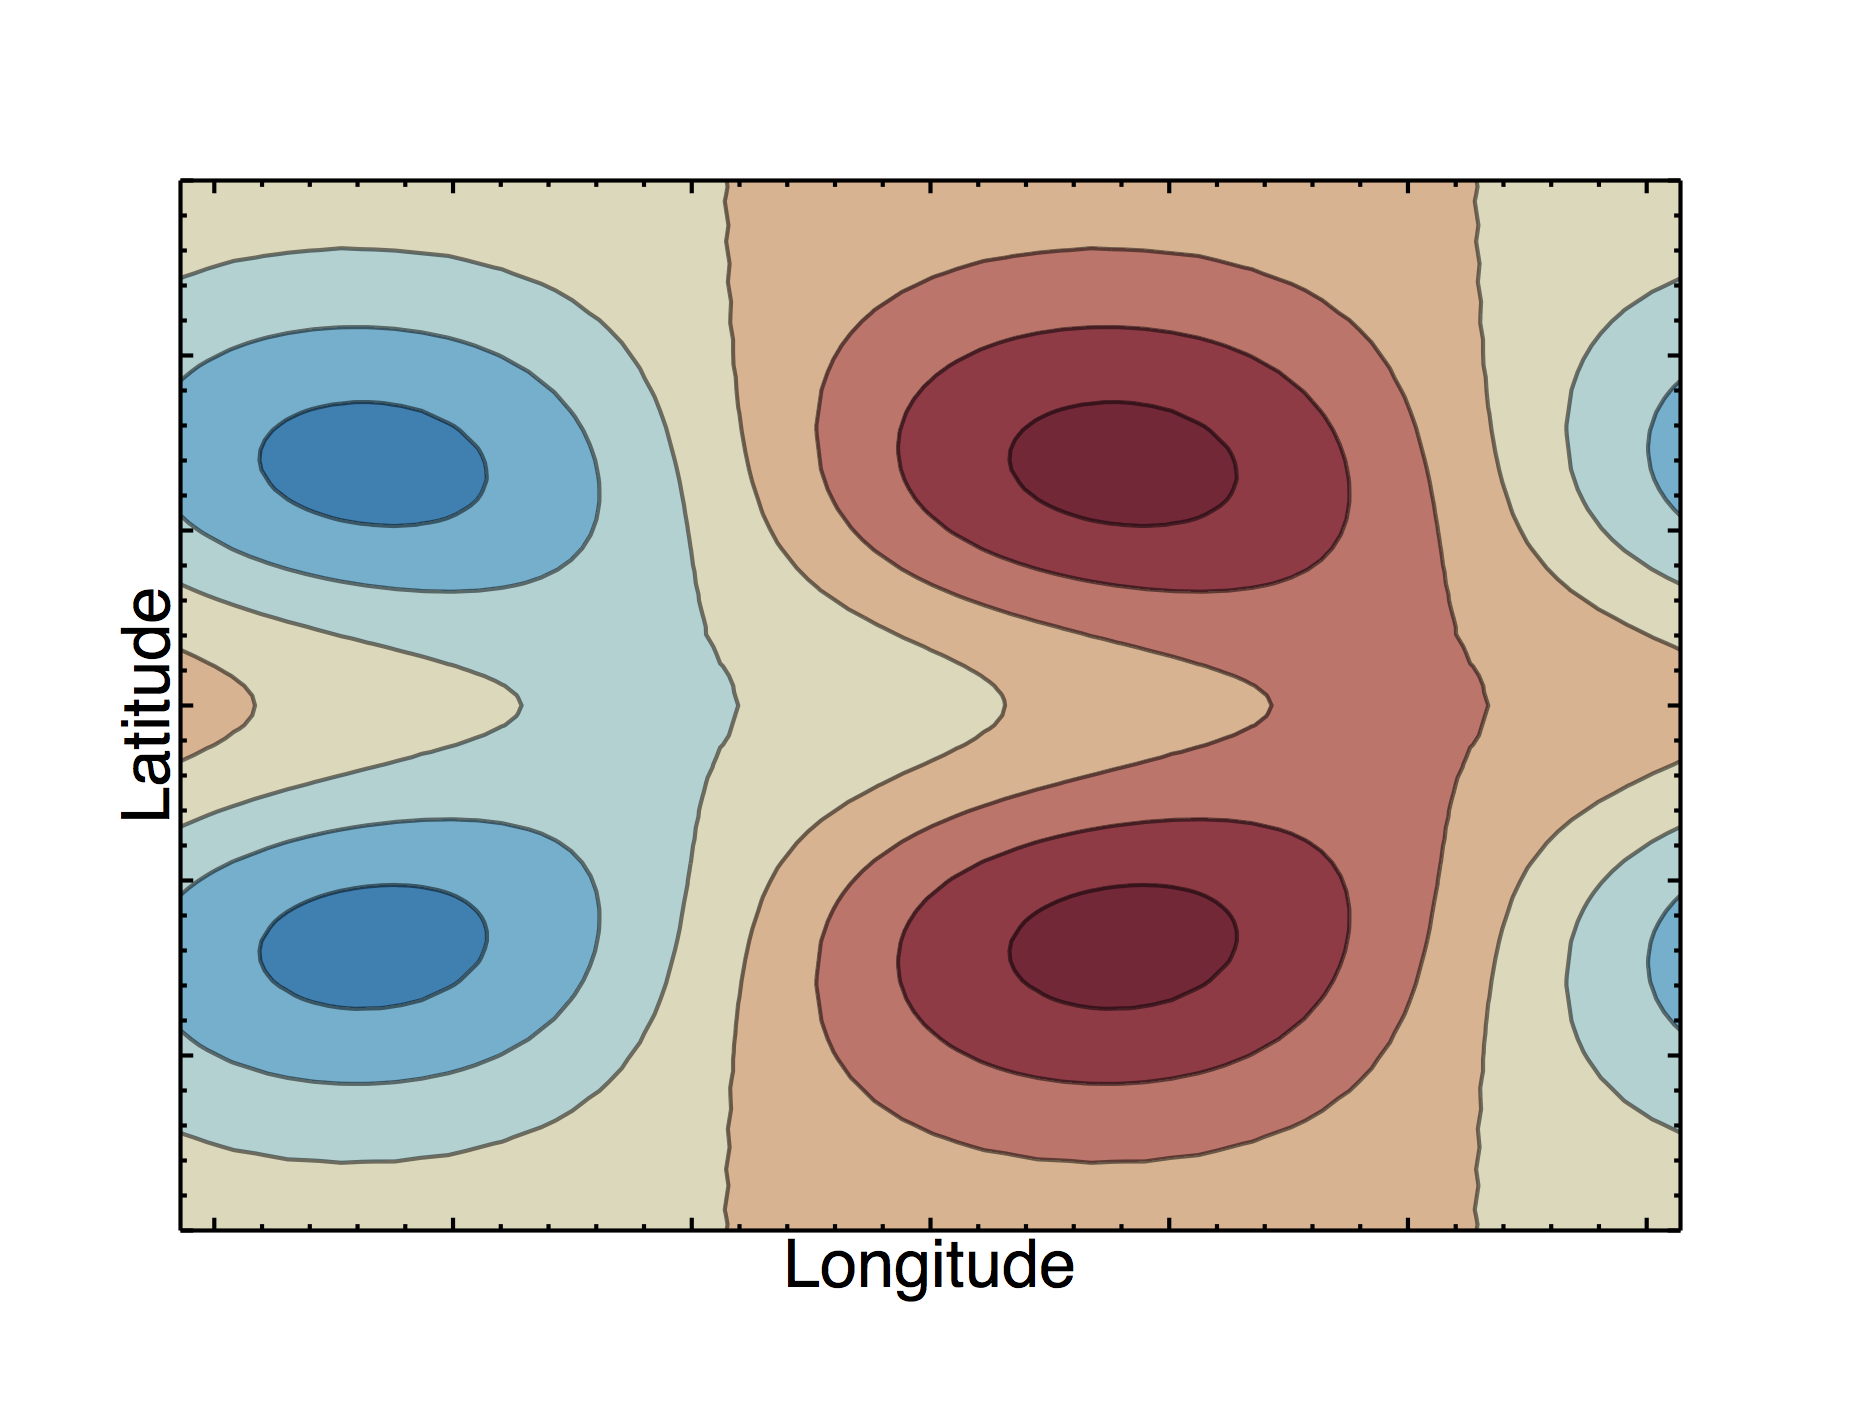
\includegraphics[width=\textwidth]{figures/wave-mean-flow/expl-shifted-matsuno.png}
    \caption{Shear Flow.}
    \label{fig:expl-shifted-matsuno}
  \end{subfigure}
  %
  \begin{subfigure}[b]{0.24\textwidth}
    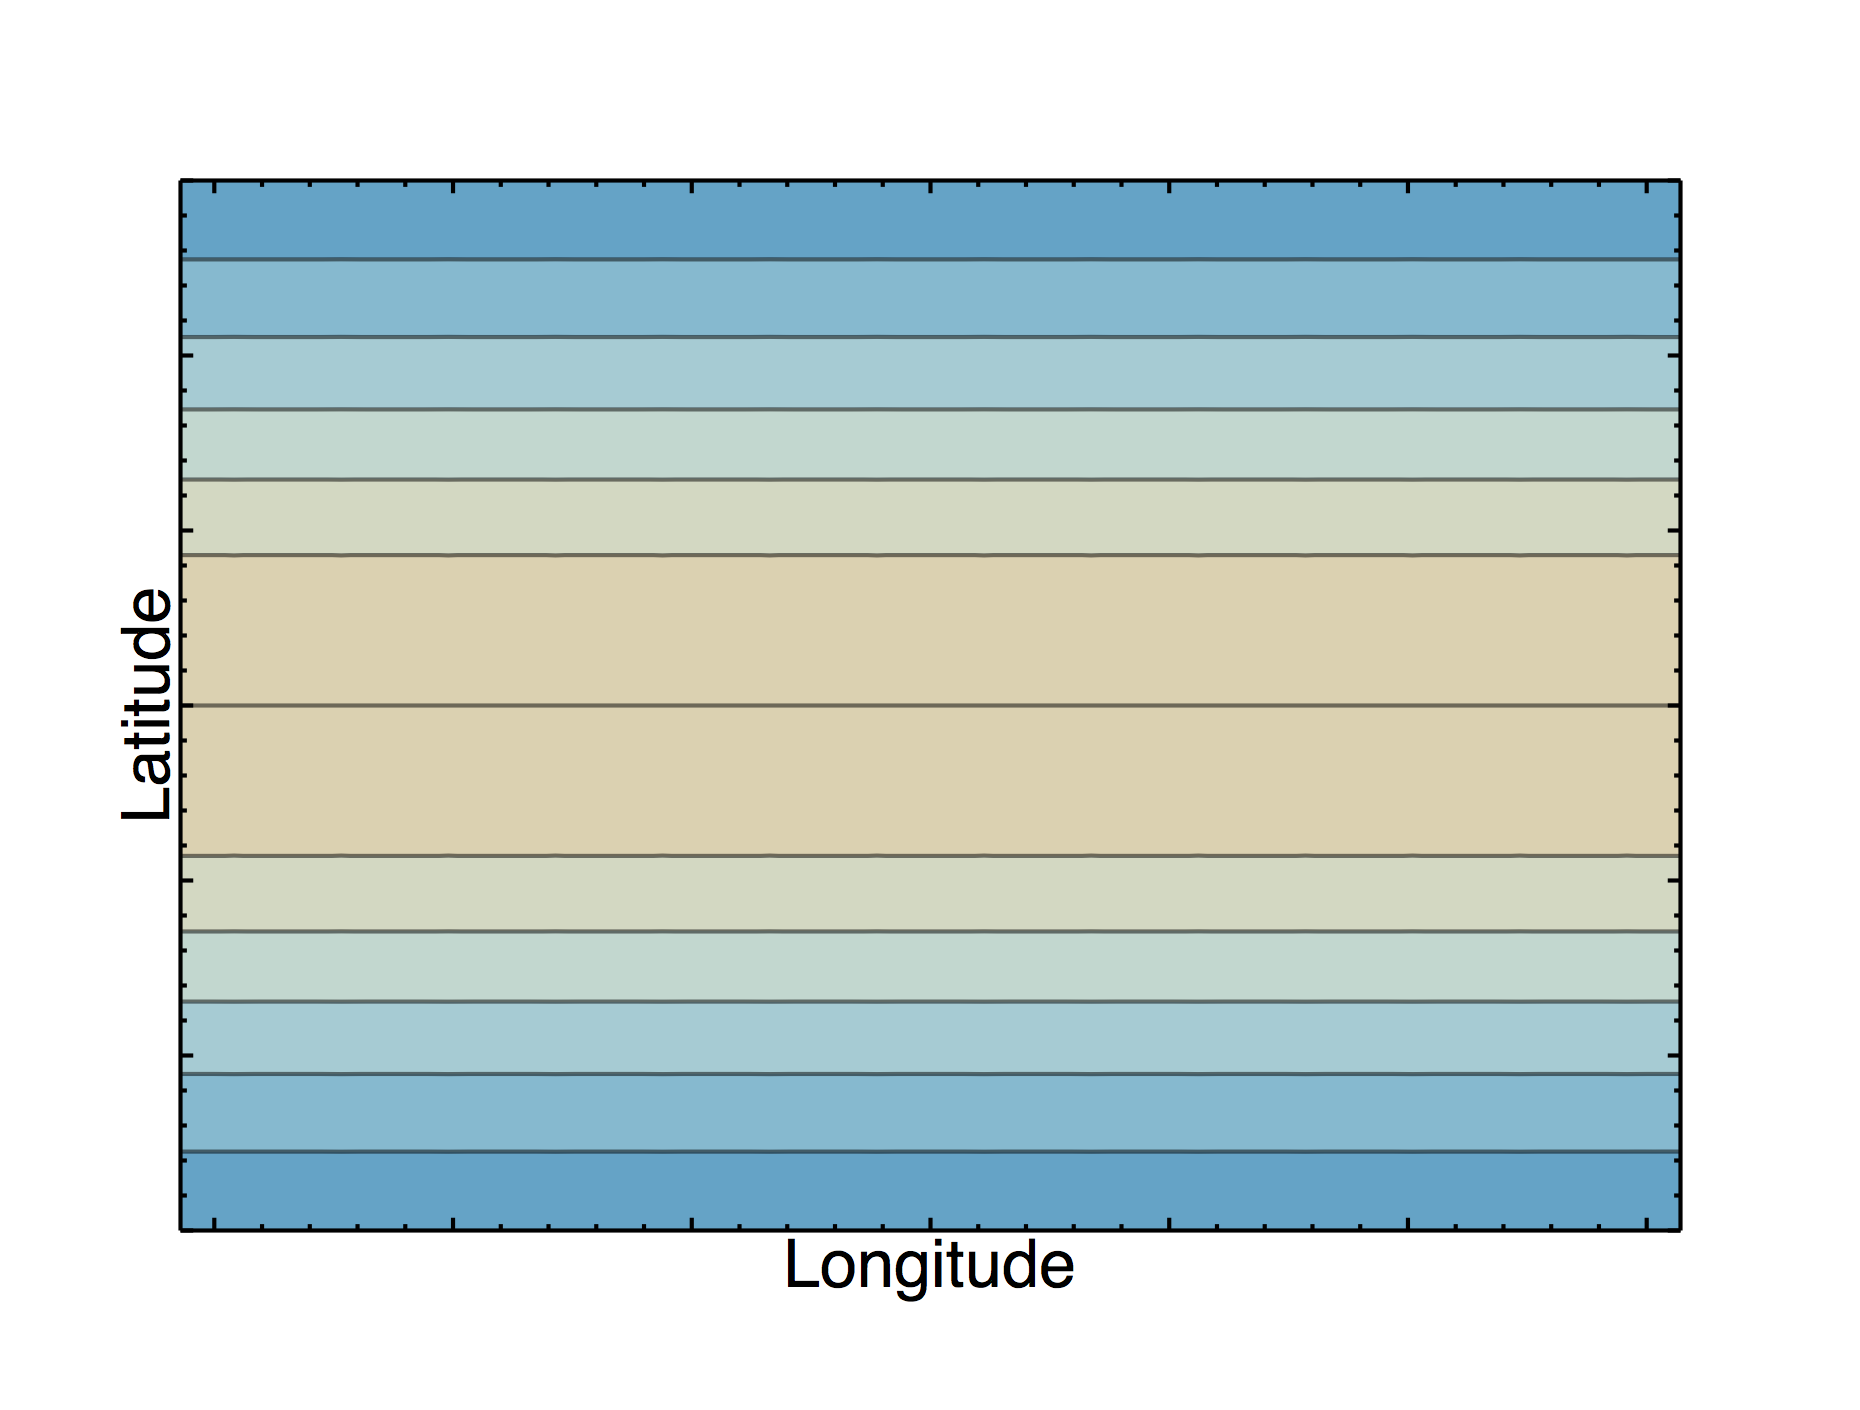
\includegraphics[width=\textwidth]{figures/wave-mean-flow/expl-phibar.png}
    \caption{Shear Flow.}
    \label{fig:expl-phibar}
  \end{subfigure}
  %
  \begin{subfigure}[b]{0.24\textwidth}
    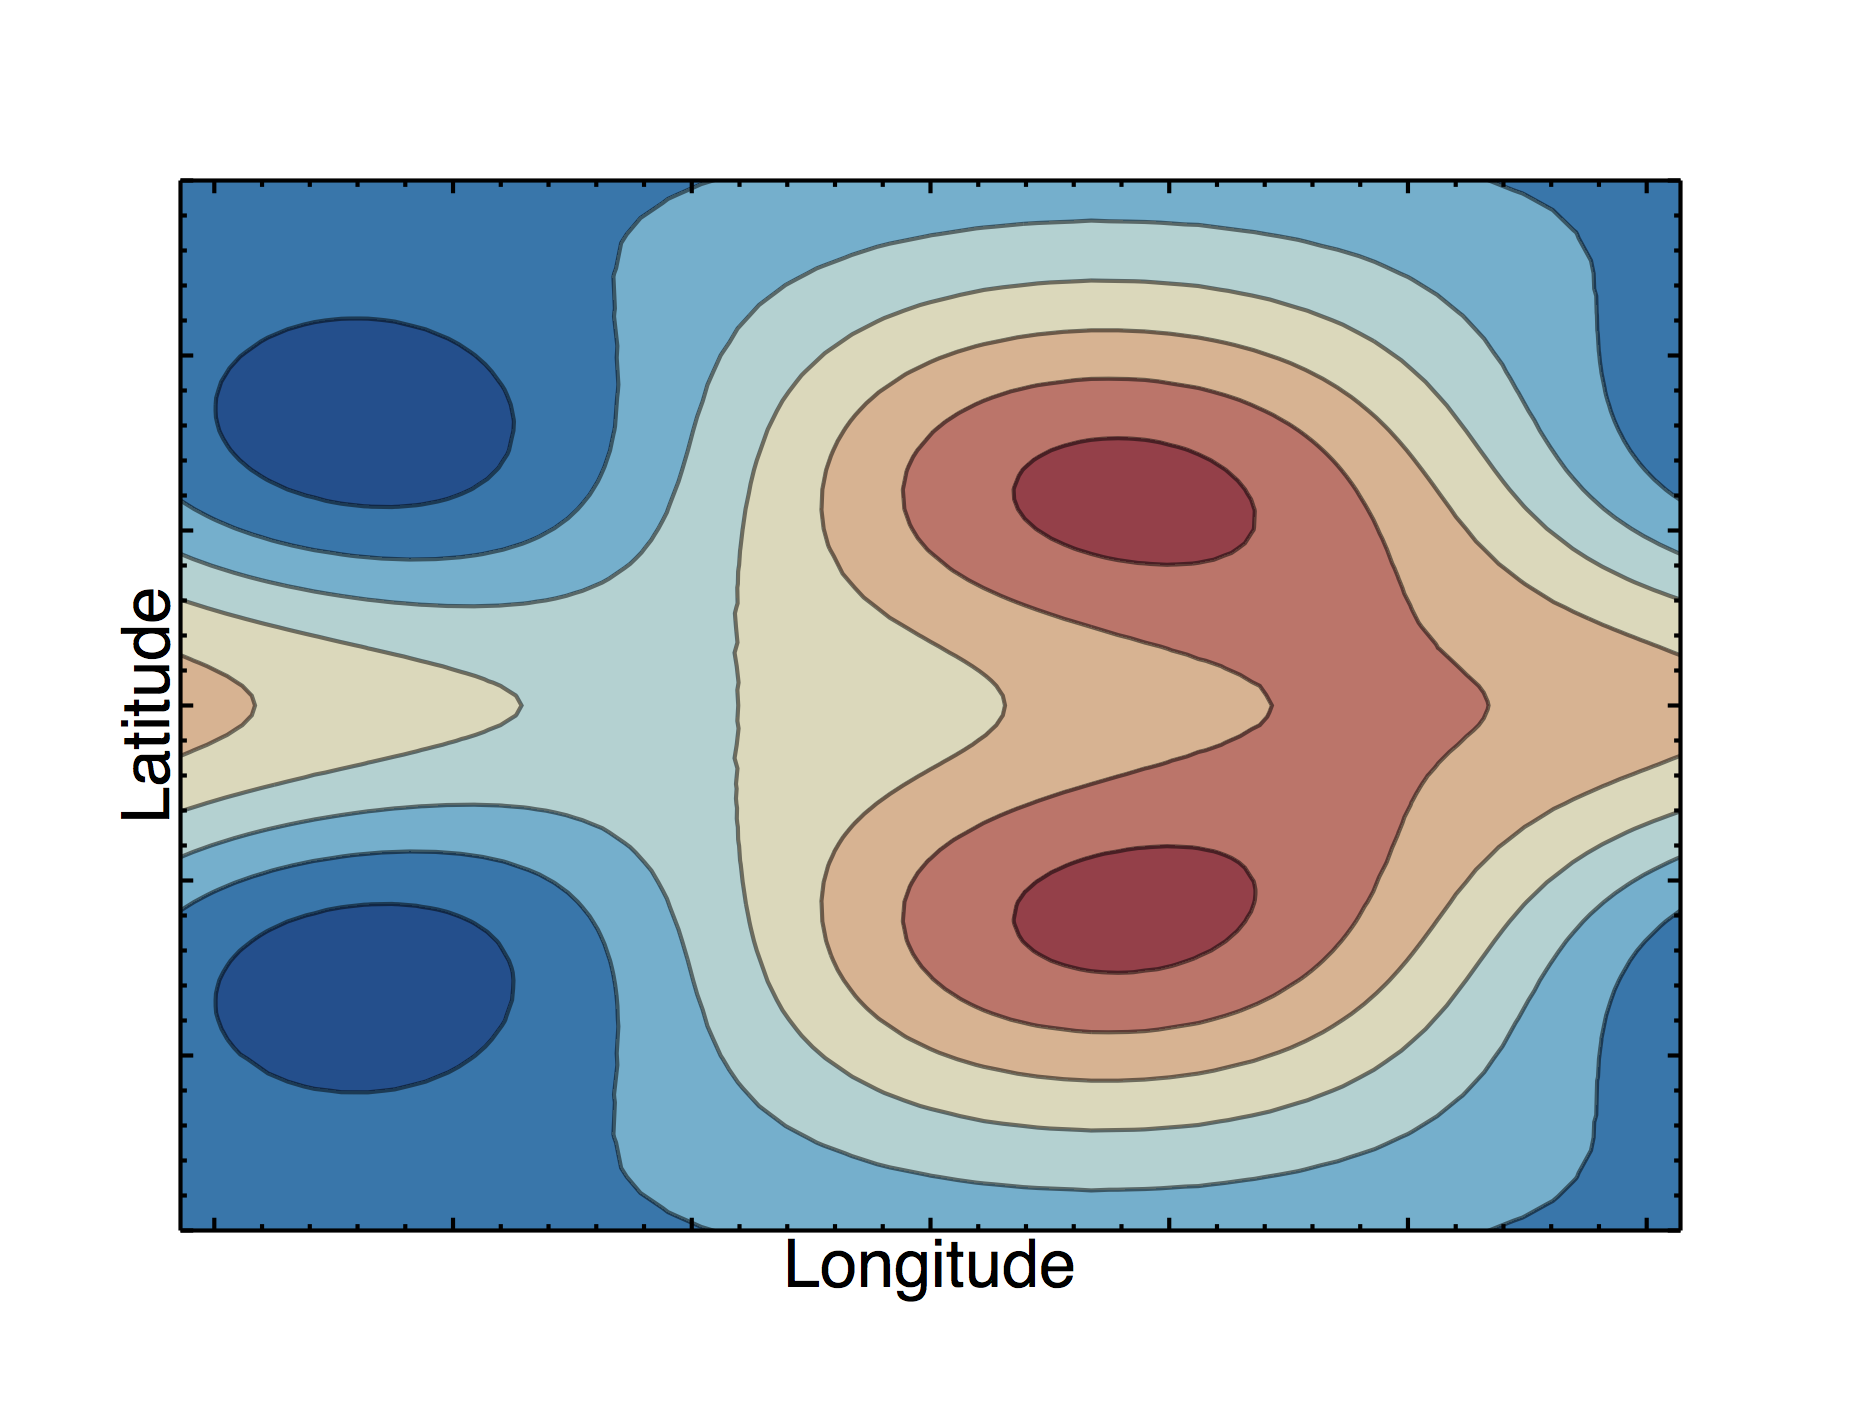
\includegraphics[width=\textwidth]{figures/wave-mean-flow/expl-plot-total.png}
    \caption{Shear Flow.}
    \label{fig:expl-plot-total}
  \end{subfigure}
  \caption{Explanation.}
  \label{fig:first-order-solutions}
\end{figure}



What is the relevance of these forced solutions for the atmospheres of tidally locked planets, and interpreting observations of them?

It is possible to match up the shifted eigenvalues of the free modes in Section X to the total forced response in Section X to understand the change in global temperature structure produced by the equatorial jet.


%SECTION CONCLUSIONS

%%%%%%%%%%%%%%%%%%%%%%%%%%%%%%%%%%%%


%SECTION 4 -- SHEAR FLOW ON BETA-PLANE AND SPHERICAL
\section{Wave Interactions with Shear Flow on a Sphere}

The beta-plane solutions are intuitive but less accurate for a sphere.



%SUBSECTION --
\subsection{Spherical Shallow-Water Equations}

%SUBSECTION --
\subsection{Forced Solutions}

\begin{figure}
  \centering
  \begin{subfigure}[b]{0.33\textwidth}
    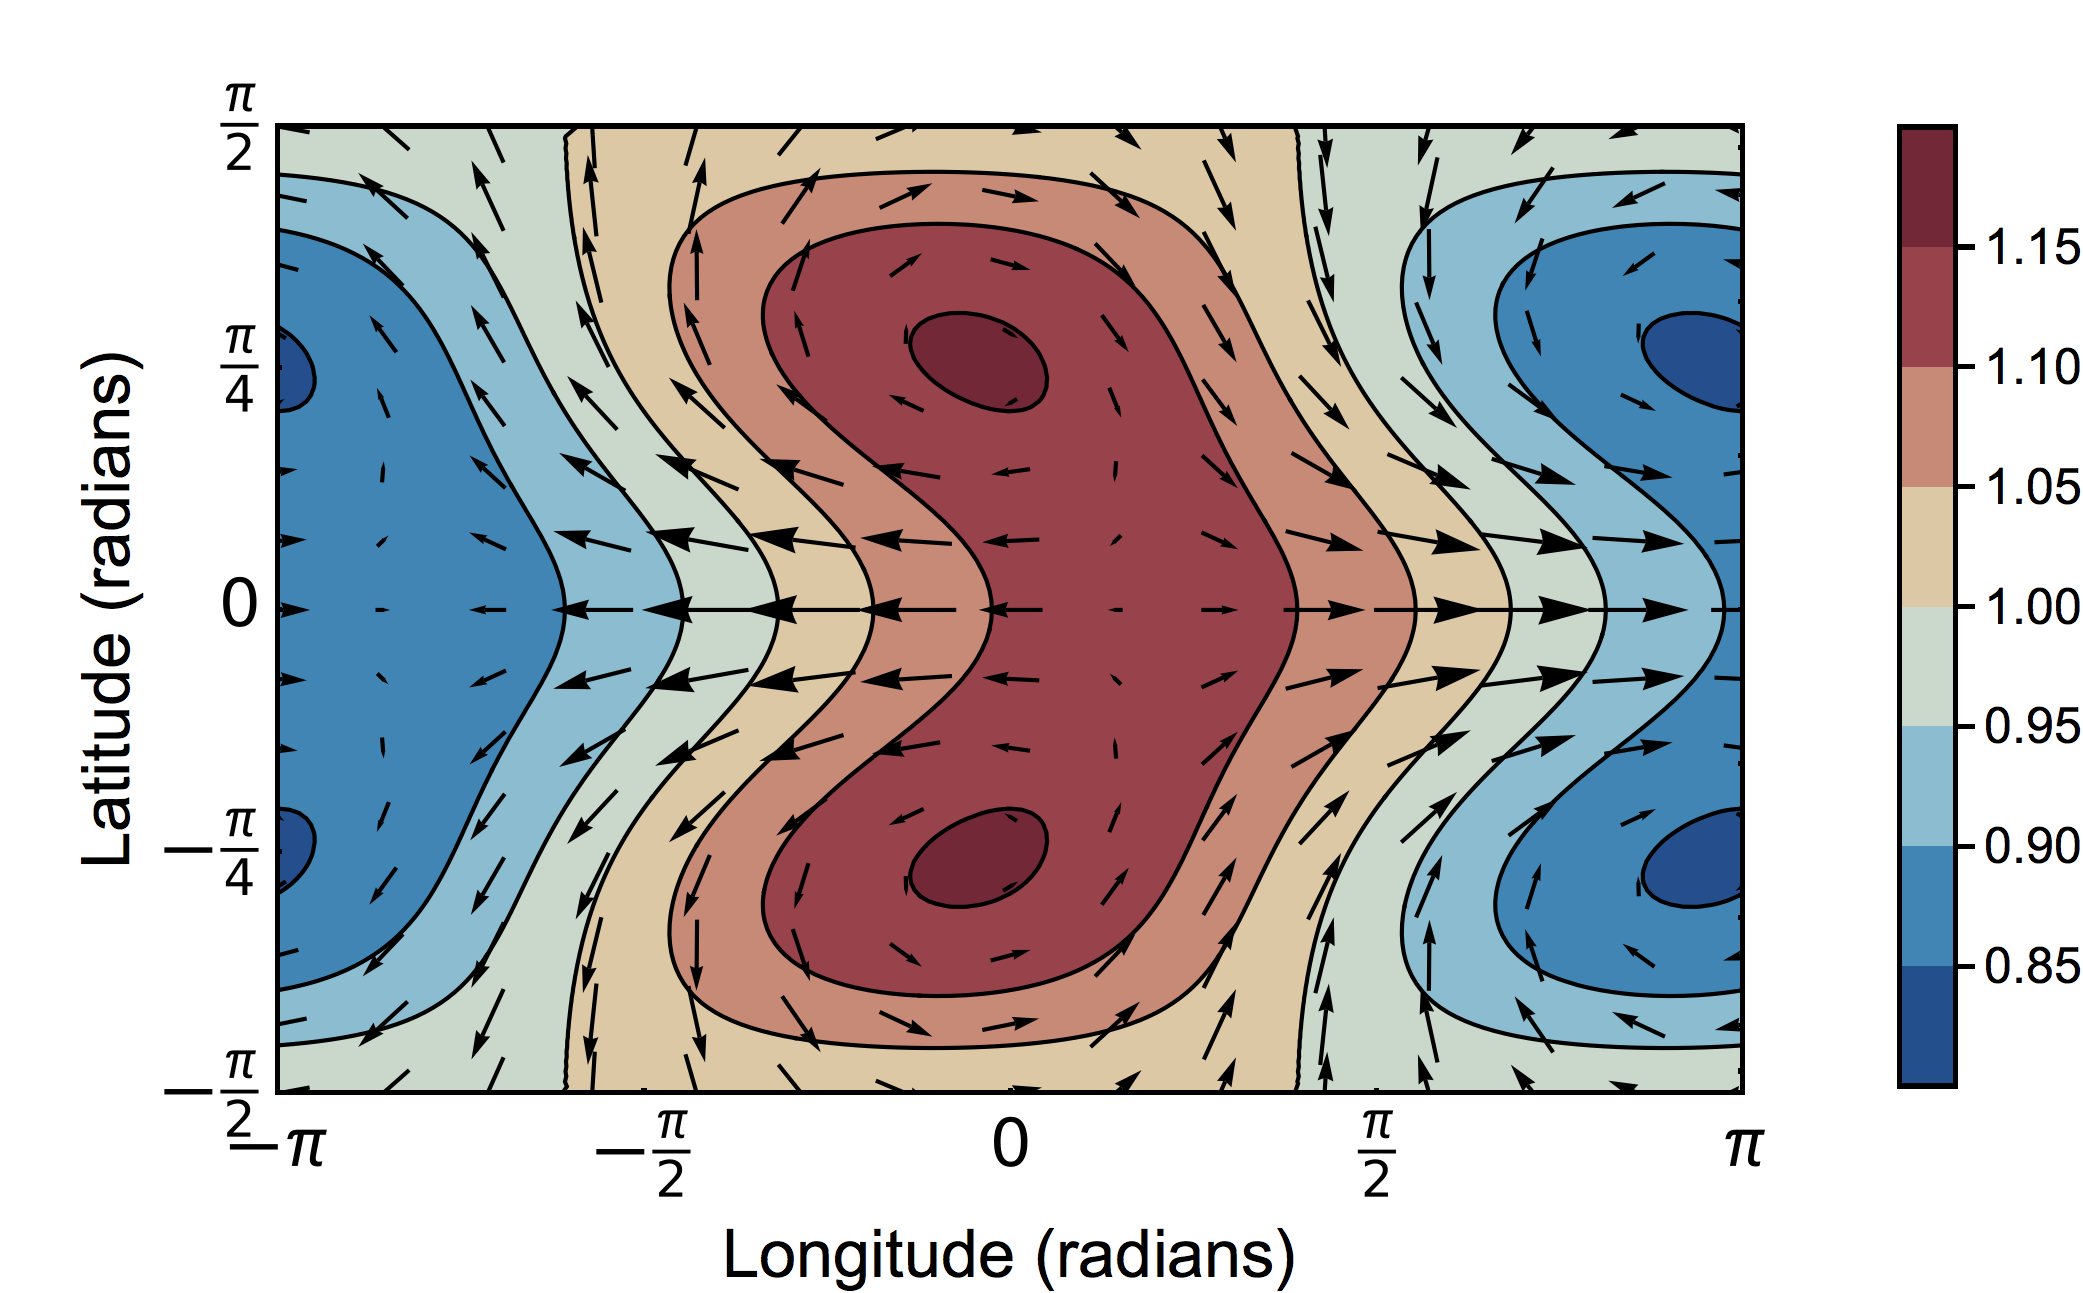
\includegraphics[width=\textwidth]{figures/wave-mean-flow/spherical-matsuno.png}
    \caption{Zero Flow.}
    \label{fig:spherical-matsuno}
  \end{subfigure}
  %
  \begin{subfigure}[b]{0.33\textwidth}
    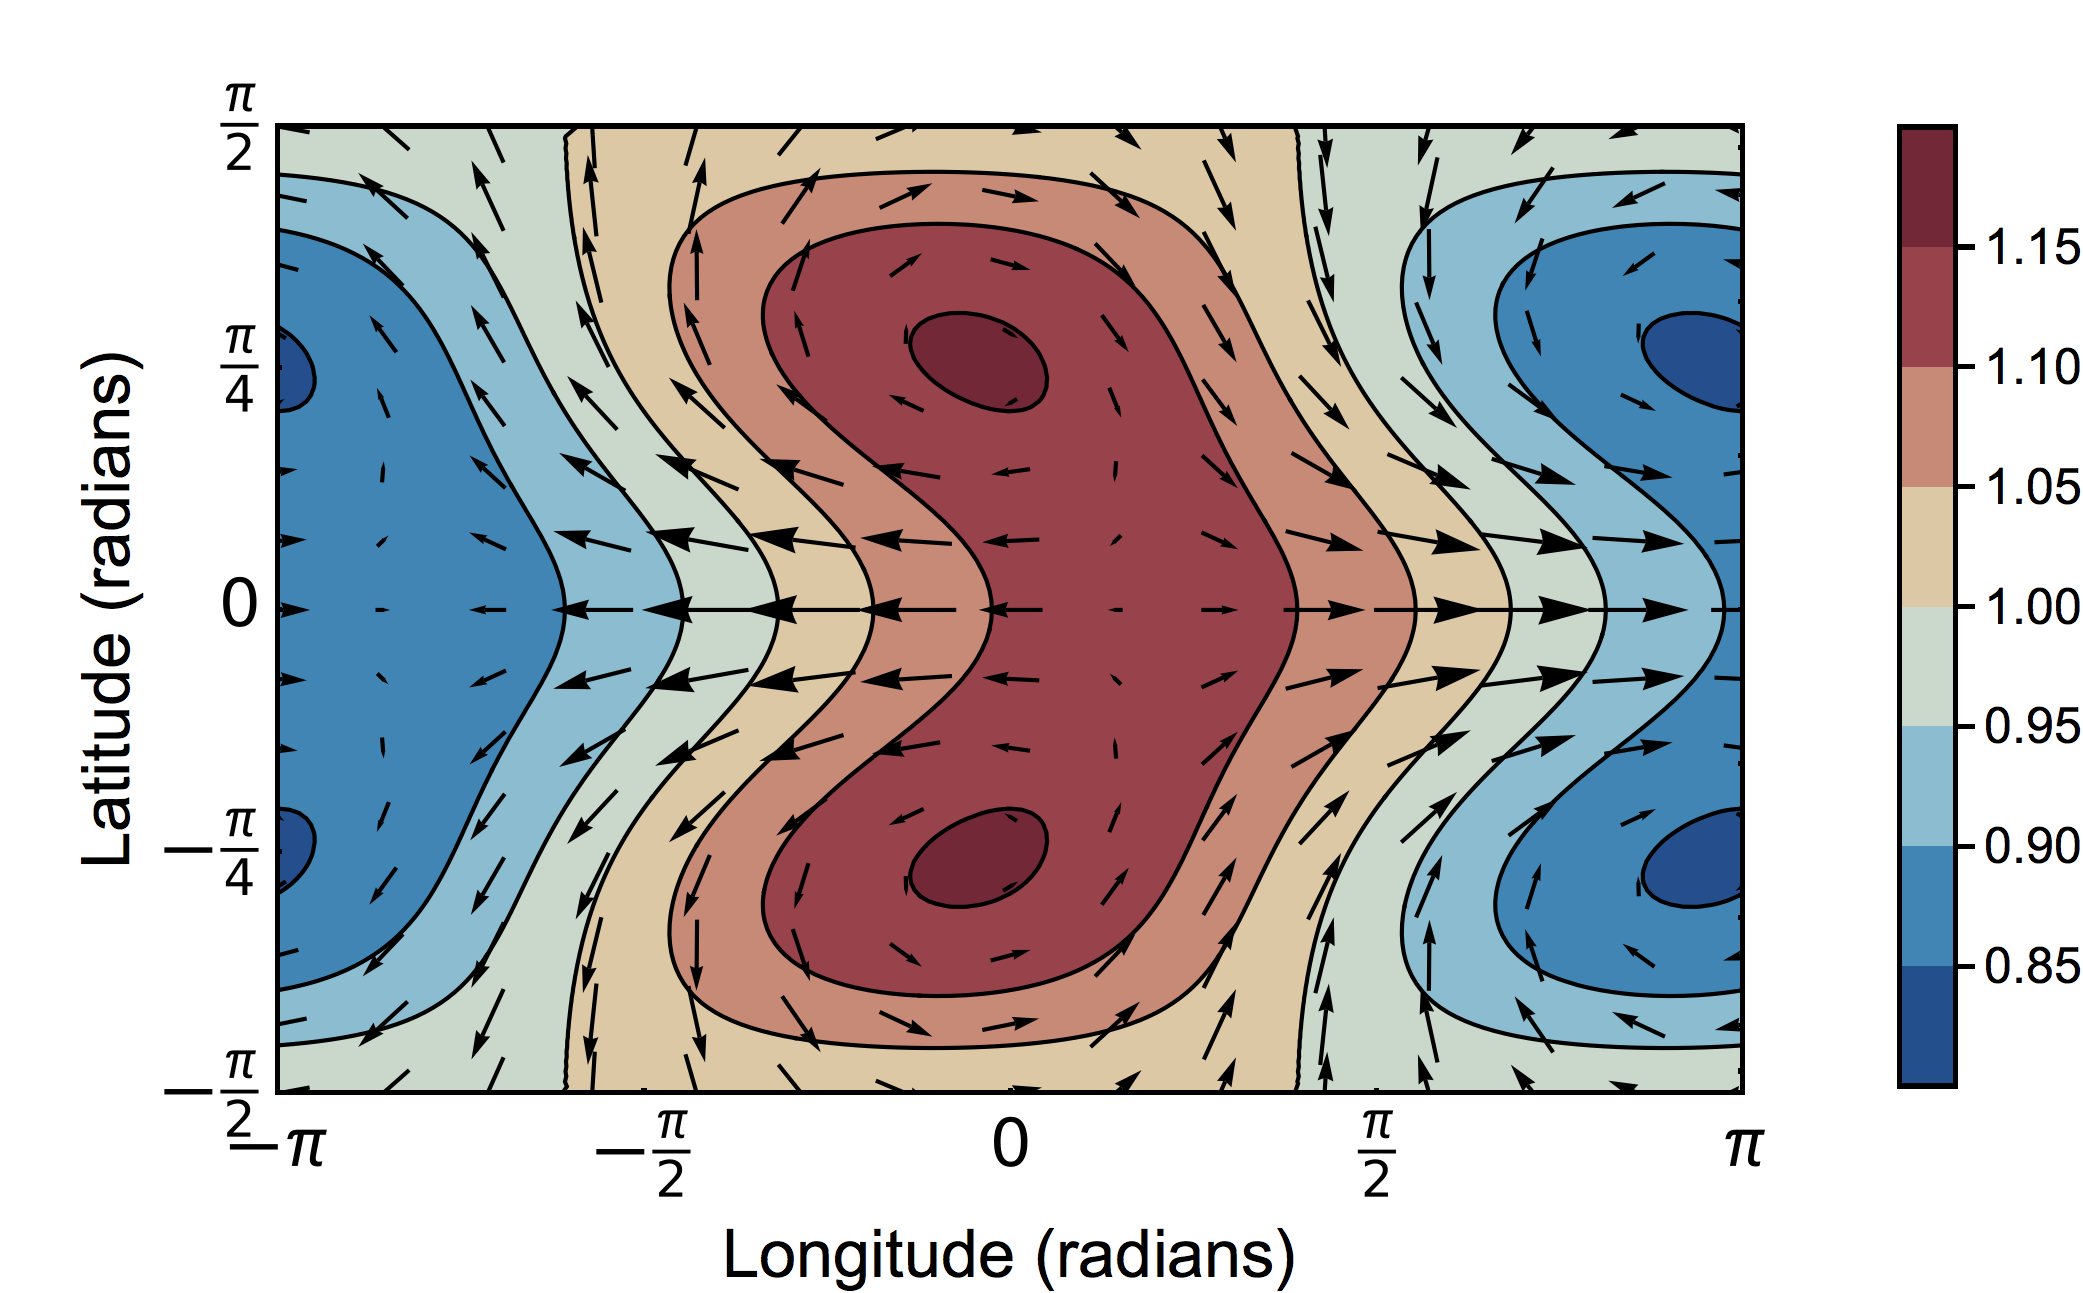
\includegraphics[width=\textwidth]{figures/wave-mean-flow/spherical-matsuno.png}
    \caption{Zero Flow.}
    \label{fig:spherical-matsuno}
  \end{subfigure}
  %
  \begin{subfigure}[b]{0.33\textwidth}
    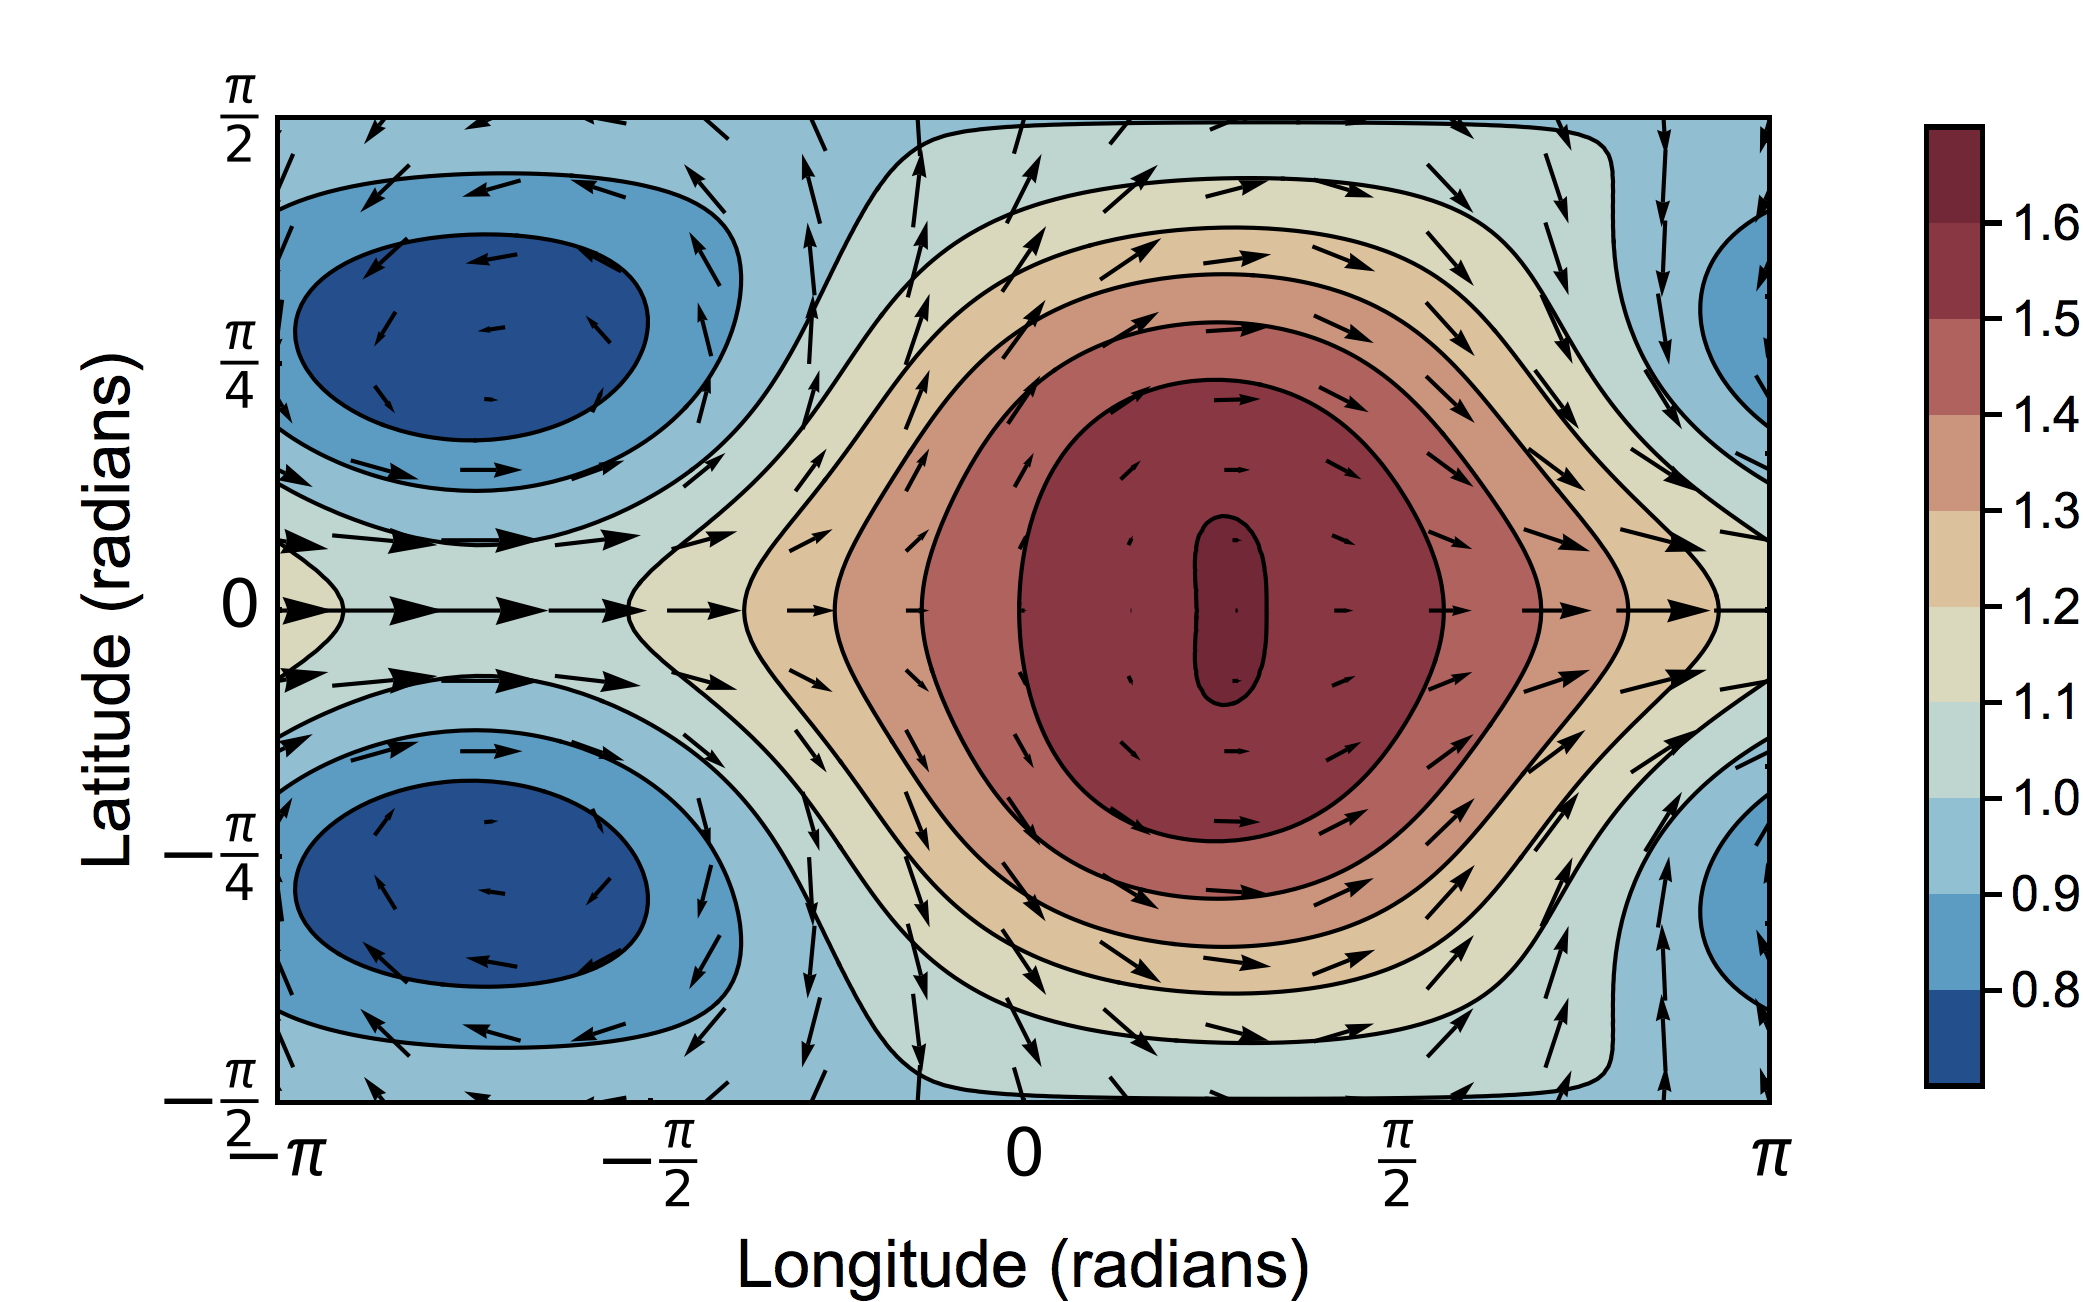
\includegraphics[width=\textwidth]{figures/wave-mean-flow/spherical-shear-2d.png}
    \caption{Zero Flow.}
    \label{fig:spherical-shear-2d}
  \end{subfigure}
  %
  \caption{Forced linear shallow-water solutions in spherical geometry with and without background shear flows. The parameters of the model are $\bar{U}=0.5 \cos\phi \exp(-(\phi/\phi_{0})^{2})$, $\phi_{0}=\pi / 3$, $\alpha_{dyn}=\alpha_{rad}=0.2$, $G=1$, $Q=0.5\cos(\phi)$, as discussed in Section \ref{sec:sphere-solutions}.}\label{fig:spherical-tests.}
  \label{fig:spherical-tests}
\end{figure}



%SECTION CONCLUSIONS

%%%%%%%%%%%%%%%%%%%%%%%%%%%%%%%%%%%%

%SECTION 5 -- SCALING RELATIONS
\section{Scaling Relations}

%SUBSECTION -- 1D SCALING
\subsection{1D Scaling Relations}

%SUBSECTION -- 2D SCALING
\subsection{2D Scaling Relations}

%SECTION CONCLUSIONS

%%%%%%%%%%%%%%%%%%%%%%%%%%%%%%%%%%%%

%SECTION 5 -- SCALING RELATIONS
\section{Other Jet Patterns}

The suite of tests in Chapter XX show that the zonal mean wind profile on a tidally locked planet is not always well represented by a Gaussian. There can be only two jets in the midlatitudes, or three jets, one on the equator.

In this section I find the forced response with different jet profiles, and show that the result is not particularly different to the Gaussian jet used up to this point.

Two Jets:

Three Jets:

One Prograde, Two Retrograde:

One Retrograde, two prograde (eddy-driven):



%%%%%%%%%%%%%%%%%%%%%%%%%%%%%%%%%%%%


%CONCLUSIONS

%RESTATE SECTION CONCLUSIONS

%OPEN OUT CONCLUSIONS



% \bibliographystyle{unsrtnat}
% \bibliography{../references.bib}
